\documentclass[a4paper]{article}

\usepackage[utf8]{inputenc}   % LaTeX, comprends les accents !
\usepackage[T1]{fontenc}      % Police contenant les caractères français
\usepackage[french]{babel}  
\usepackage{fullpage}
\usepackage{graphicx}
\usepackage{wrapfig}
\usepackage{float}
\usepackage{blindtext}
\usepackage{algorithm2e}
% \usepackage[open,openlevel=1]{bookmark}
\usepackage[colorlinks=true,linkcolor=black,urlcolor=black,bookmarksopen=true,bookmarksnumbered=true]{hyperref}
\usepackage{bookmark}
\usepackage{blindtext}
% \usepackage{biblatex}

\RestyleAlgo{ruled}
\graphicspath{ {./img/} }

\begin{document}
	\title{Reconnaissance de l'écriture manuscrite\\Rapport de projet}
	\author{Laurent Antoinette, Romain Campillo, Tony Nguyen\\\emph{L3 informatique}\\
	Faculté des Sciences\\
	Université de Montpellier.}
	\date{\today}
	\maketitle
	\thispagestyle{empty}
	\begin{figure}[h]
		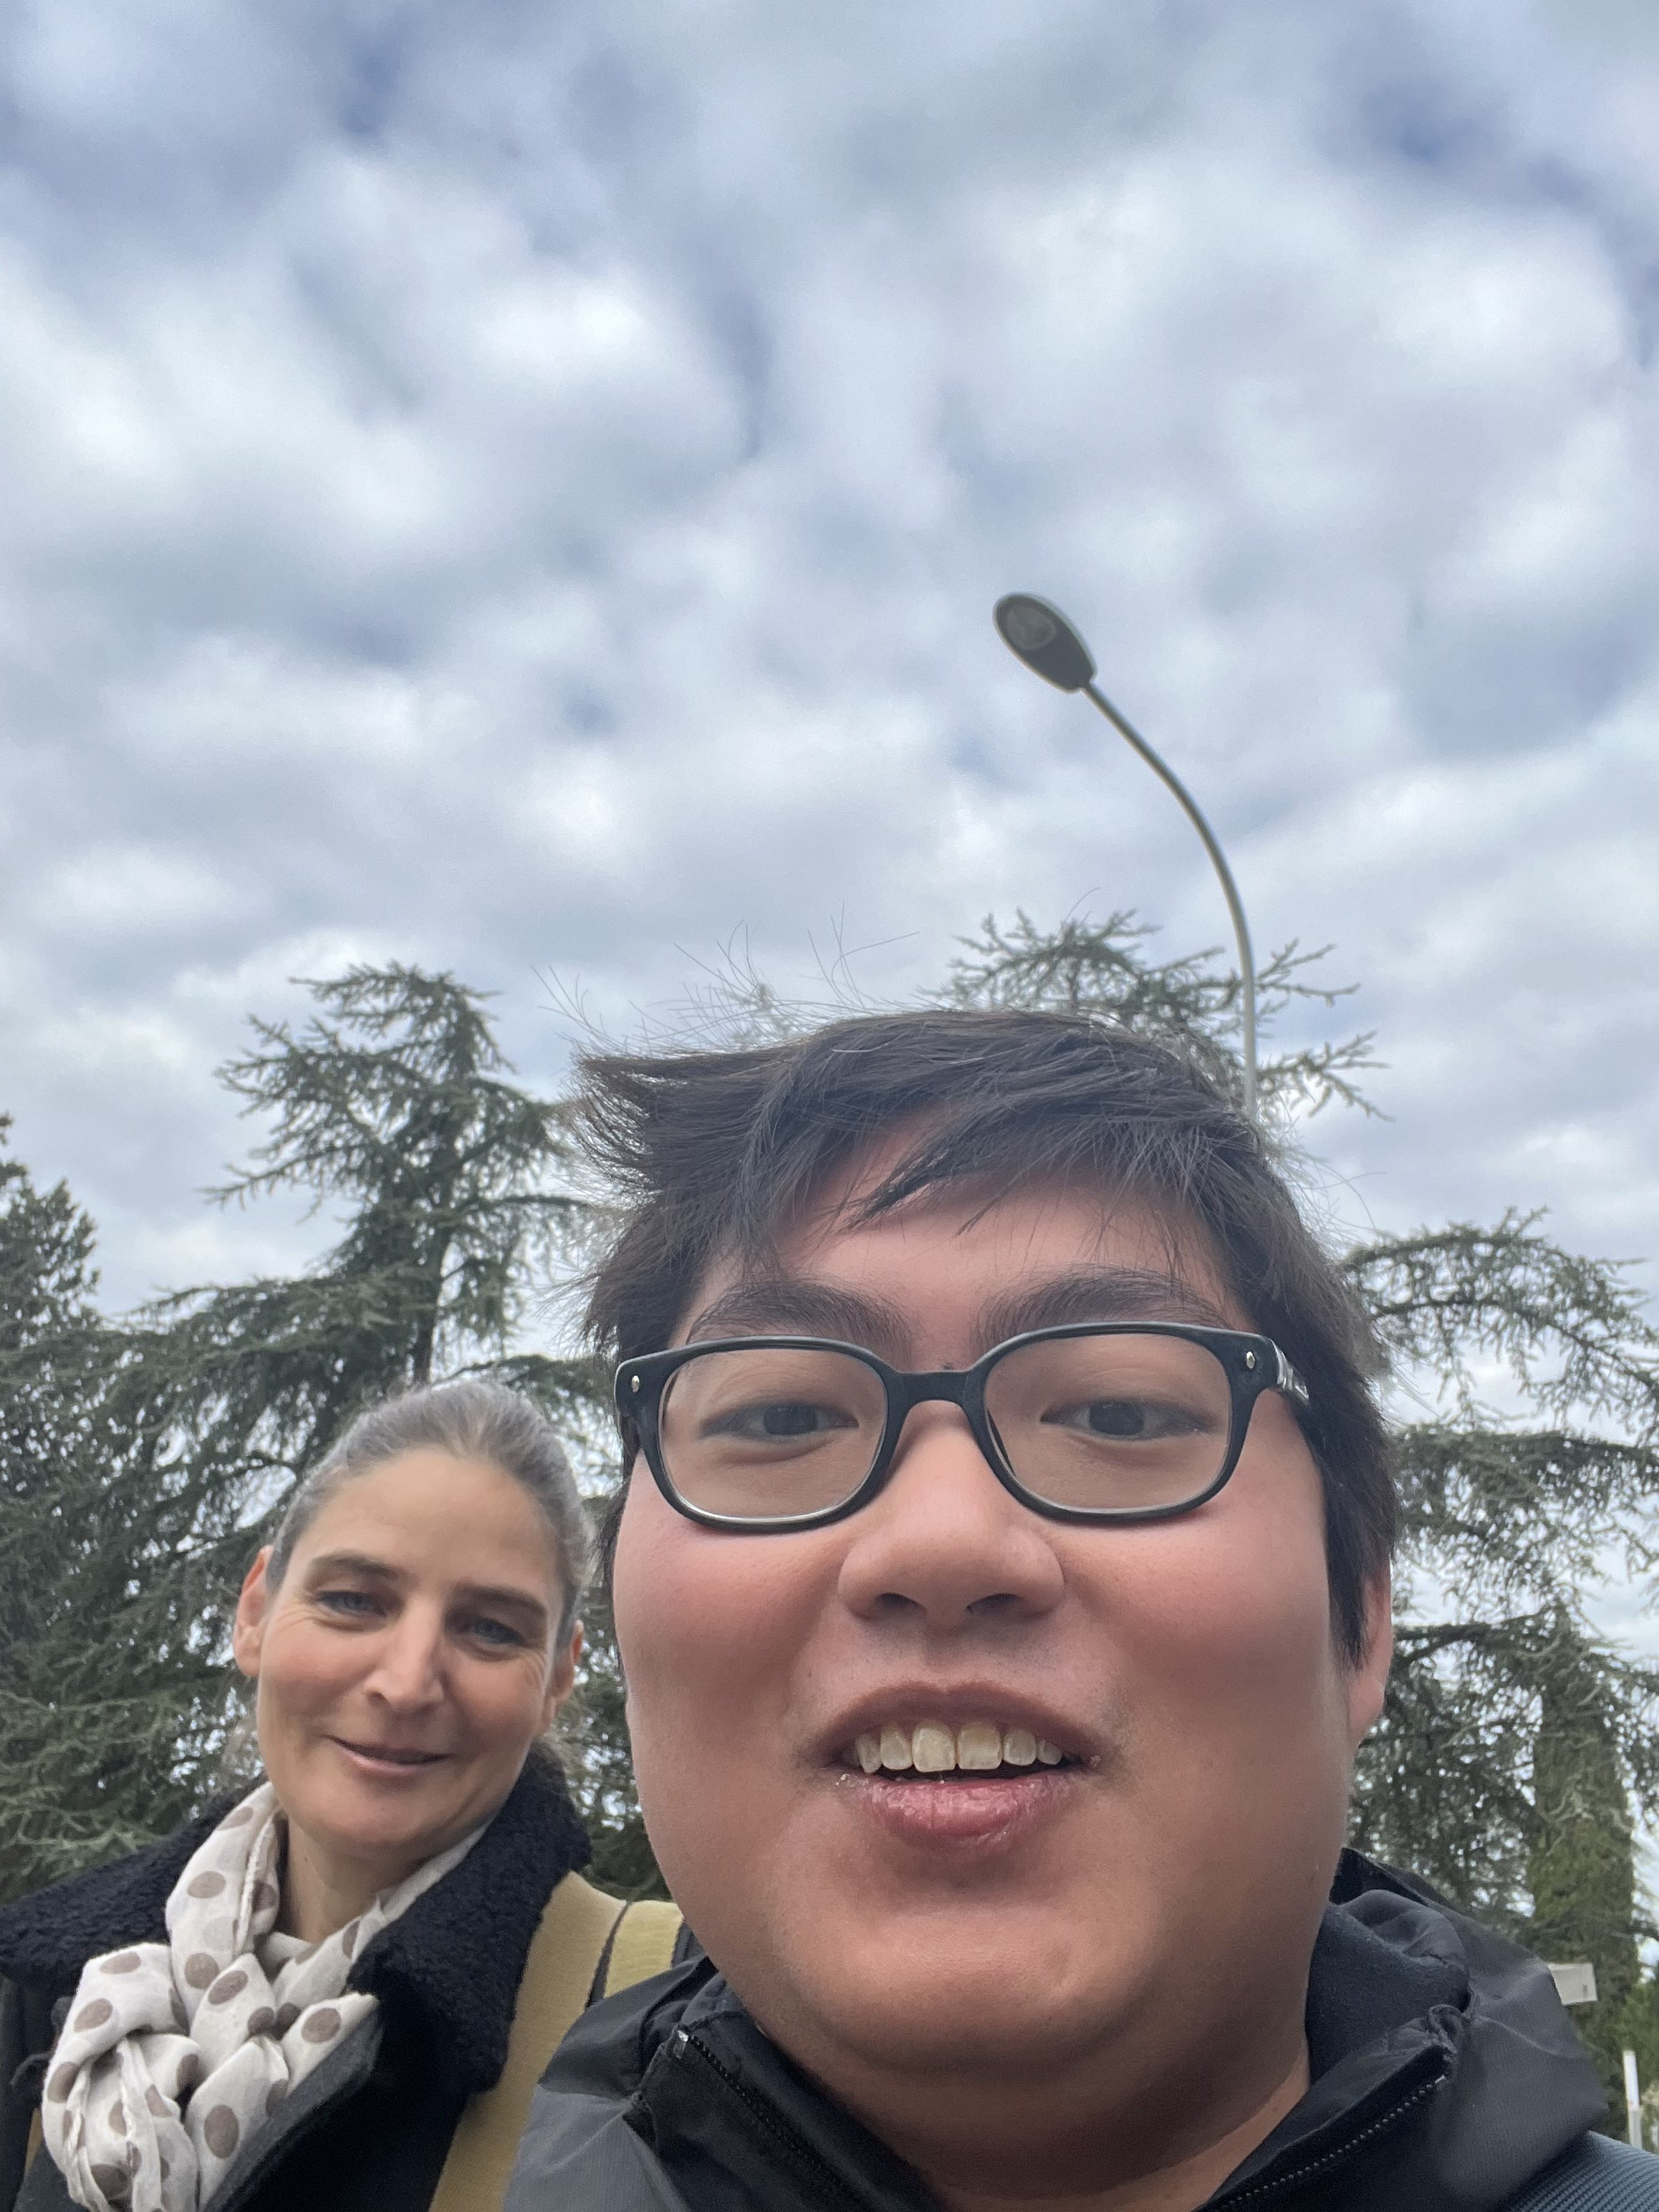
\includegraphics[scale=.1]{selfie_tony_clementine.jpg}
		% 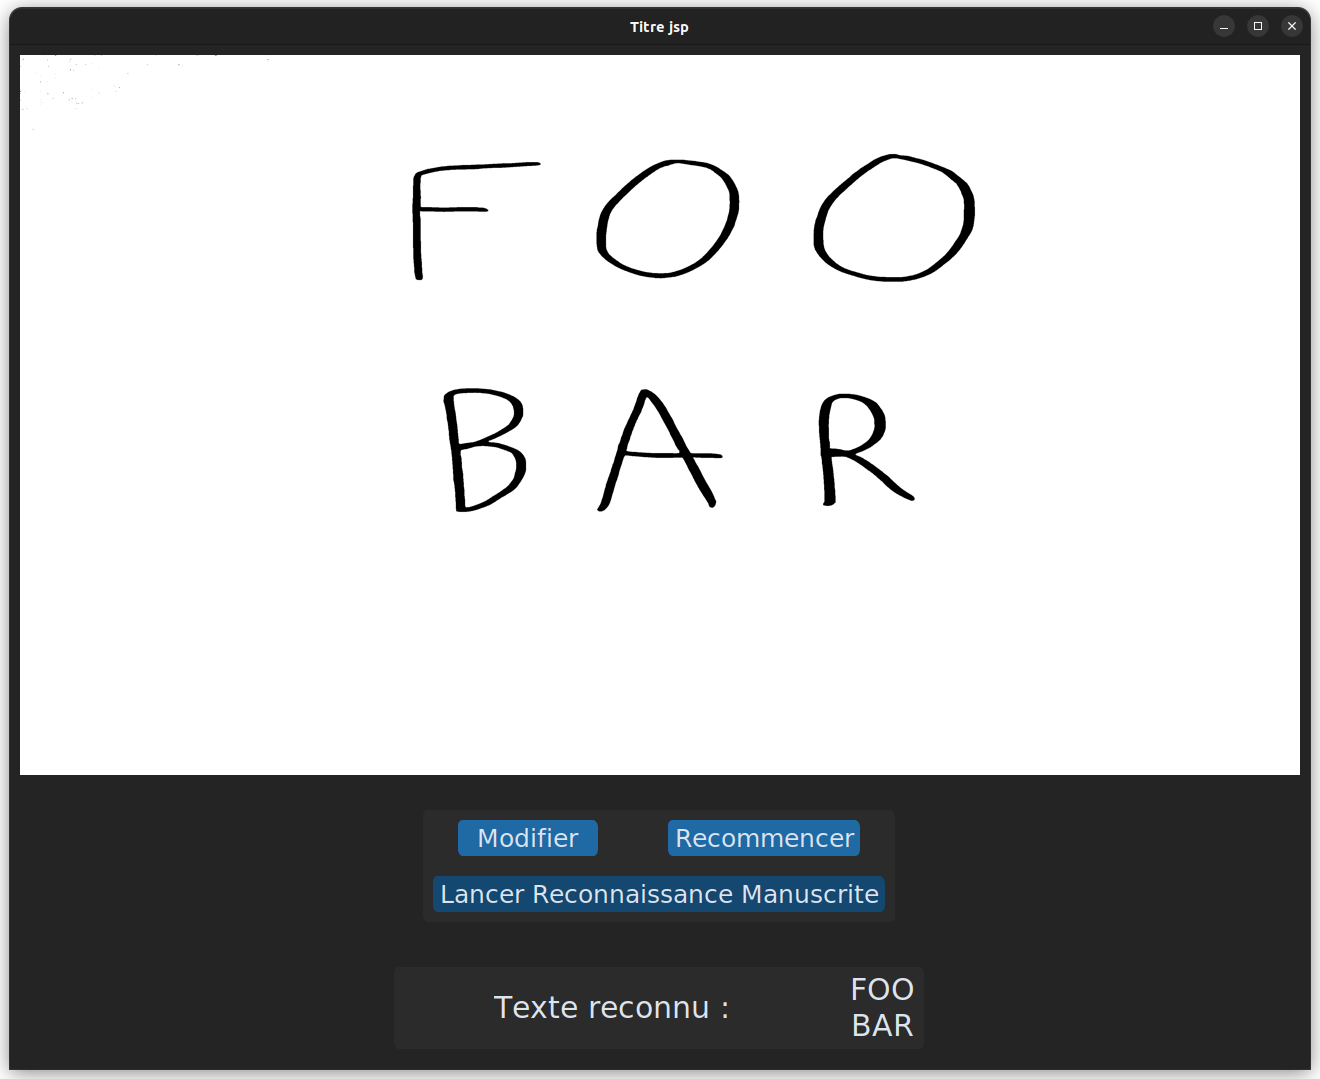
\includegraphics[width=\textwidth]{recon.png}
		\centering
	\end{figure}
	\newpage
	\thispagestyle{empty}
	\tableofcontents
	\newpage
	\thispagestyle{empty}
	\listoffigures
	\listofalgorithms
	\newpage
	\section{Présentation du Sujet } 
		\subsection{La problématique}
			\paragraph{}
				La reconnaissance de l'écriture manuscrite consiste à traduire un texte manuscrit en un texte numérique, interprétable par l'ordinateur. Bien que cette application commence à être utilisé dans différents secteurs, 
				la variation des styles d'écritures manuscrites d'une personne à l'autre et la mauvaise qualité du texte pose des défis importants pour leurs numérisations.% manuscrits en texte numérique.%  convertion en texte numérique.
\\Les méthodes classiques étudiées auparavant ou présentées dans la littérature, notamment l'amélioration de la qualité d'images (filtres, etc) ou la reconnaissance des formes complexes, peuvent ne pas répondre à ce type de problématique.
\\Ainsi dans ce projet, nous allons explorer un autre axe de recherche basée sur les méthodes de réseaux de neuronne qui ont prouvé leur efficacité à reconnaître et classifier les formes les plus complexes.
\\Cette recherche va nous permettre de mettre en oeuvre nos compétences en traitement d'image et d'explorer de nouvelles méthodes plus avancées.

			% L'essence du problème est qu'un texte dans un document est très diffrent d'une photo du même document. Dans le 1er cas, le format rend le contenu comprehensible par un ordinateur, il peut donc 
			% chercher un mot dans le texte ou le modifier pour corriger des fautes d'orthographe. Dans le 2e cas, l'image représente la même chose. MAIS, la machine ne comprend le sens de l'information 
			% représentée. Il voit les pixels mais pas les charactères. De plus, des imperfections dans la capture du document changent la photo (ex: luminosité, angle ...), il y a une modification des informations
			% alors que le texte ne change pas.
			% \\Réussir à lire du texte sur des images permettrait de faciliter la numérisation de document papier. Ainsi, libérer les Humains de quelques tâches redondantes. Lire des formulaires ou encore d'améliorer les moteurs de recherche avec des images qui contient du texte sont des applications possibles.
		\subsection*{}
			Le traitement automatique de l'information numérique est particulièrement intéressant pour des étudiants en informatique car il peut être abordé de nombreuses manières. 

			jsp mais faut reformuler
			% L'utilisation de l'intelligence artificielle et notamment des réseaux de neurones permettrait de reconnaitre facilement les formes
			% Grâce à la croissance exponentielle de l'intelligence artificielle ces dernières années,
			% nous pouvons 
			%  En effet, un projet sur le traitement automatique de l'information numérique est exactement ce que des étudiants en informatique devraient faire. Nous avons pu constater une explosion
			% de l'intelligence artificielle ces dernières années, notamment les réseaux neuronaux. À l'heure actuelle, ils sont capables de détecter des objets et de les classifier. Ce projet est tout à fait 
			% intéressant pour de futurs étudiants en master IASD.
		\subsection{Quelques approches de reconnaissance de formes}
			\subsubsection{k-Nearest Neighbor}
				La méthode du k-Nearest Neighbor se base sur le principe que les échantillons appartenant à la même classe ont tendance à se regrouper dans l'espace des caractéristiques.
				Pour classifier une nouvelle entrée, on regarde les k points d'entraînement les plus proches. La nouvelle entrée est classée en fonction de la classe majoritaire des voisins
				% Méthode statistique, il y a un plan avec plein d'objets qui forment des troupeaux, notre lettre est quelque part dans le plan, on trace un cercle autour, notre lettre est identifiée comme l'objet présent au plus grand nombre à l'intérieur du cercle.
			\subsubsection{Template matching} 
				% En gros, comparaison de l'image avec la base de donnée entière à l'aide d'une fonction de distance. 
				\paragraph{}
					Cette approche est l'une des plus simple. Voici en quoi elle consiste :\\Nous allons partir d'une banque d'image de référence. À chaque fois que nous souhaitons classifier une nouvelle image, nous allons comparer cette nouvelle image avec toute nos images de référence à l'aide d'une simple fonction de distance euclidienne.
				\paragraph{} L'avantage de cette solution est qu'il n'est pas nécessaire d'entrainer un modèle au préalable. Elle est néanmoins sensible aux rotations et aux déplacements dans l'image.%si la nouvelle image subit une rotation trop grande,
			\subsubsection{Les réseaux de neuronnes} 
				Les réseaux de neuronnes sont souvent utilisés pour résoudre des problèmes de classification et de prédiction.
				Ils sont constitués de couches de neurones interconnectés en s'inspirant du fonctionnement du cerveau humain.
				Cette méthode nécessite une phase d'apprentissage qui peut être longue, coûteuse et qui repose sur la qualité et la quantité des données d'entraînement fournies.
				Nous avons choisi cette solution pour reconnaitre les lettres dans notre projet.

		\subsection{Cahier des charges}

			\subsubsection{Objectifs}
			Notre objectif est de proposer une méthode pour convertir une image de texte manuscrit en un texte numérique.\\
			Dans notre étude nous allons considérer les 26 lettres de l'alphabet latin en majuscule et espacées.


			\subsubsection{Besoins et contraintes}
				\paragraph{Les besoins}
					\subparagraph{Capturer une image}
						L'utilisateur pourra prendre des photos par notre logiciel à l'aide d'une webcam. Mais il pourra également utiliser des images depuis son système de fichier. Tout cela à travers une interface Homme-Machine.
					\subparagraph{Pré-traitement}
						Le logiciel réduira le bruit et rendra l'image plus nette à l'aide de plusieurs filtres prédéfinis. 
					\subparagraph{Segmentation de l'image}
						Les différents caractères présents sur l'image seront localisés à l'aide d'histogramme de projection.
					\subparagraph{Extraction des caractères}
						Les caractères seront ensuite découpés pour former leurs propres imagettes i.e. une image qui contient TEST devriendra 4 petites imagettes contenant respectivement T E S T.
					\subparagraph{Reconnaissance}
						Les imagettes feront l'objet d'une reconnaissance de façon individuelle. La solution que nous choisissons d'implémenter est un réseau neuronal convolutif.
					\subparagraph{Présenter}
						Une fois que les imagettes sont reconnues en caractère. Il est nécessaire de les assembler et d'afficher à l'utilisateur les mots reconnus.
				\paragraph{Les contraintes}
					Nous nous fixons comme contraintes de ne pas utiliser de services comme Google Collab car Google possède un modèle économique type "Freemium" (initialement gratuit mais avec des fonctinalités payantes). Nous souhaitons créer un logiciel suffisament performant pour qu'il puisse être lancé sur l'une de nos machines personelles. \\De plus, une webcam est nécessaire, ou alors un appareil photo numérique.
			\subsubsection{Résulats attendus}
				\paragraph{}
					Notre programme doit reconnaître des lettres manuscrites sur un fond blanc. Les lettres seront des caractères majuscules non-liés et sans accents ni caractères spécials.
	\section{Technologies utilisées} 
		\subsection{Langages et outils}
			\subsubsection{Python3}
				Python3 est un langage de programmation interprété, multiparadigme et multiplatformes. Il favorise la programmation impérative structurée, fonctionnelle et orientée objet. Il est doté d'un typage dynamique fort, d'une gestion automatique de la mémoire par ramasse-miettes et d'un système de gestion d'exceptions. (\url{https://fr.wikipedia.org/wiki/Python_(langage)})
				\paragraph{} Nous avons choisi ce langage car il est simple à comprendre et relativement facile à lire. De plus, par sa popularité, de nombreuses bibliothèques implémentent ce dont nous avons besoin. Python étant conçu pour programmer rapidement et efficacement, nous pourrons nous concentrer davantage sur l'implémentation (à redire).

				% Test \cite{textbook}
				% \cite{web:lang:python}
			\subsubsection{OpenCV}
				\begin{wrapfigure}{r}{0.15\textwidth}
					
\includegraphics[width=0.15\textwidth]{OpenCV.png}
				\end{wrapfigure}
				OpenCV (Open Computer Vision) est une bibliothèque open source spécialisée dans le traitement d'images en temps réel.
				Elle est déposée sous licence libre, et sa popularité ainsi que sa simplicité d'utilisation en font un outil adéquat pour notre projet.
				Parmi ses nombreuses fonctionnalités, nous utiliserons surtout ses fonctions de filtrage et de seuillage.
				
				\newline
			\subsubsection{You Only Look Once}
				\paragraph{}
				You Only Look Once (YOLO) est une archicture de Réseau Neuronal Convolutif (CNN) qui est capable de localiser des objets dans une image et, en même temps, de les classifier.

				\paragraph{Les réseaux de neurones}
					Les réseaux de neurone simulent plus ou moins le fonctionnement du cerveau humain. Ils sont constitués d'une multitude de neurones interconnectés entre eux qui reçoivent et renvoient des informations.
					\subparagraph{} Un neurone prend plusieurs entrées pondérées, les somme, puis les passe à travers une fonction d'activation pour produire une sortie vers un autre neurone.
					\subparagraph{} L'architecture des réseaux de neurone simple est organisée en couche. La 1ère couche représente l'entrée et la dernière couche la sortie.
					Entre le début et la fin du réseau, les couches intermédiaires sont connectées vers l'avant et de façon complète. Un neurone est connecté à tous les neurones de la couche précédente et de la suivante mais pas à ceux de la même couche.
					L'apprentissage d'un réseau de neurones en couches se fait par rétropropagation, où l'erreur entre la sortie du réseau et la sortie attendue est propagée en arrière dans le réseau, et les poids des connexions entre les neurones sont ajustés pour minimiser cette erreur.
					Ce processus est répété pour chaque exemple d'entraînement jusqu'à ce que le réseau atteigne un niveau de précision satisfaisant.	
						
					\subparagraph{Les Réseaux de Neurones Convolutifs (CNN)} 
					Contrairement aux réseaux de neurones traditionnels, qui utilisent des connexions denses entre les neurones des couches adjacentes, les CNN utilisent des couches de convolution qui appliquent des filtres pour extraire des caractéristiques importantes de l'image.
					Cette opération permet d'extraire des motifs et des formes à différentes échelles et positions de l'image.
					Les couches de sortie du CNN sont des couches denses classiques qui combinent les informations extraites par les couches précédentes pour produire une sortie finale, telle que la classe de l'objet présent dans l'image.

					\subparagraph{} YOLO est connu pour sa grande précision et ses bonnes performances dans la détection des objets dans une scène. Etant donné que nous localisons déjà les lettres dans notre image, nous n'utiliserons cependant que les fonctionnalités de classification de YOLO, qui nous suffisent amplement.

	\newpage
	\section{Développements Logiciel : Conception, Modélisation, Implémentation}
		\begin{figure}[h]
			\centering
			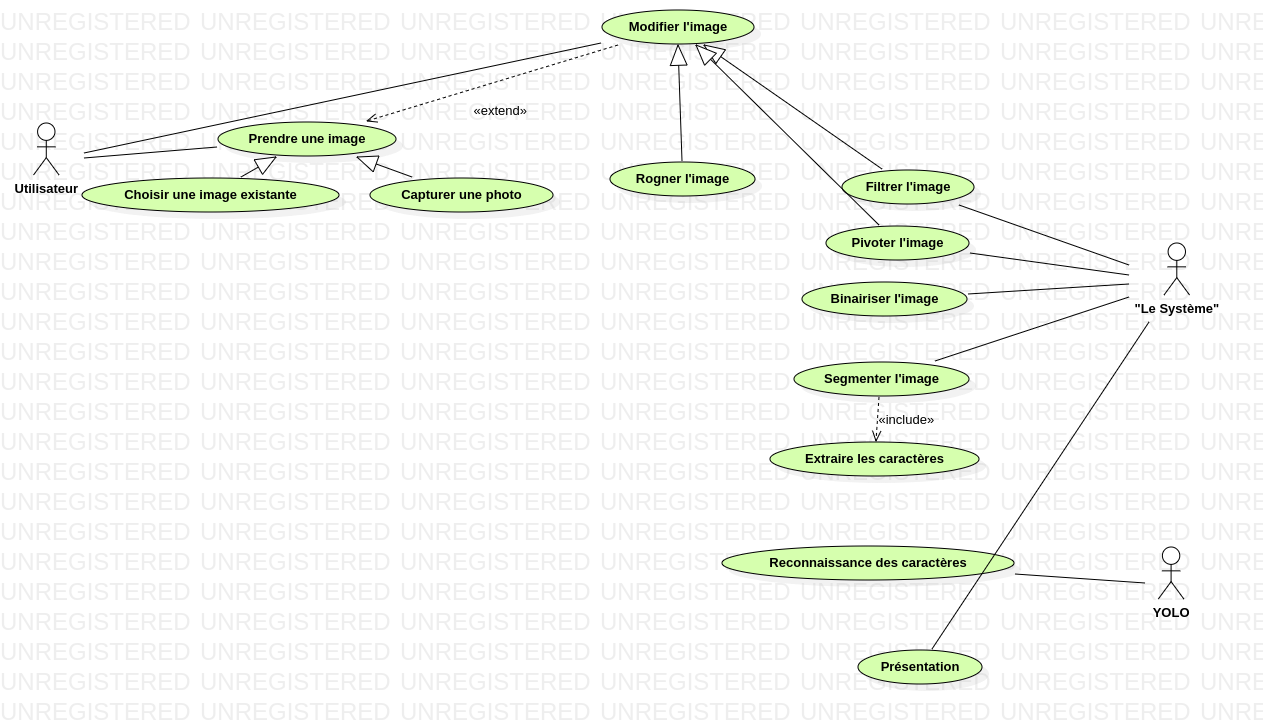
\includegraphics[width=\textwidth]{UseCaseDiagram.png}
			\caption{Diagramme de cas d'utilisation}
			\label{fig:useCaseDiagram}
		\end{figure}


		\subsection{Interface Homme-Machine}
			L'IHM nous permet de prendre des photos avec une webcam connectée à l'ordinateur ou choisir à partir d'une fenêtre une image déjà existante. 
%Diagramme de Cas d'Utilisation à la page \pageref{fig:useCaseDiagram}. 
			\begin{figure}[H]
				\centering
				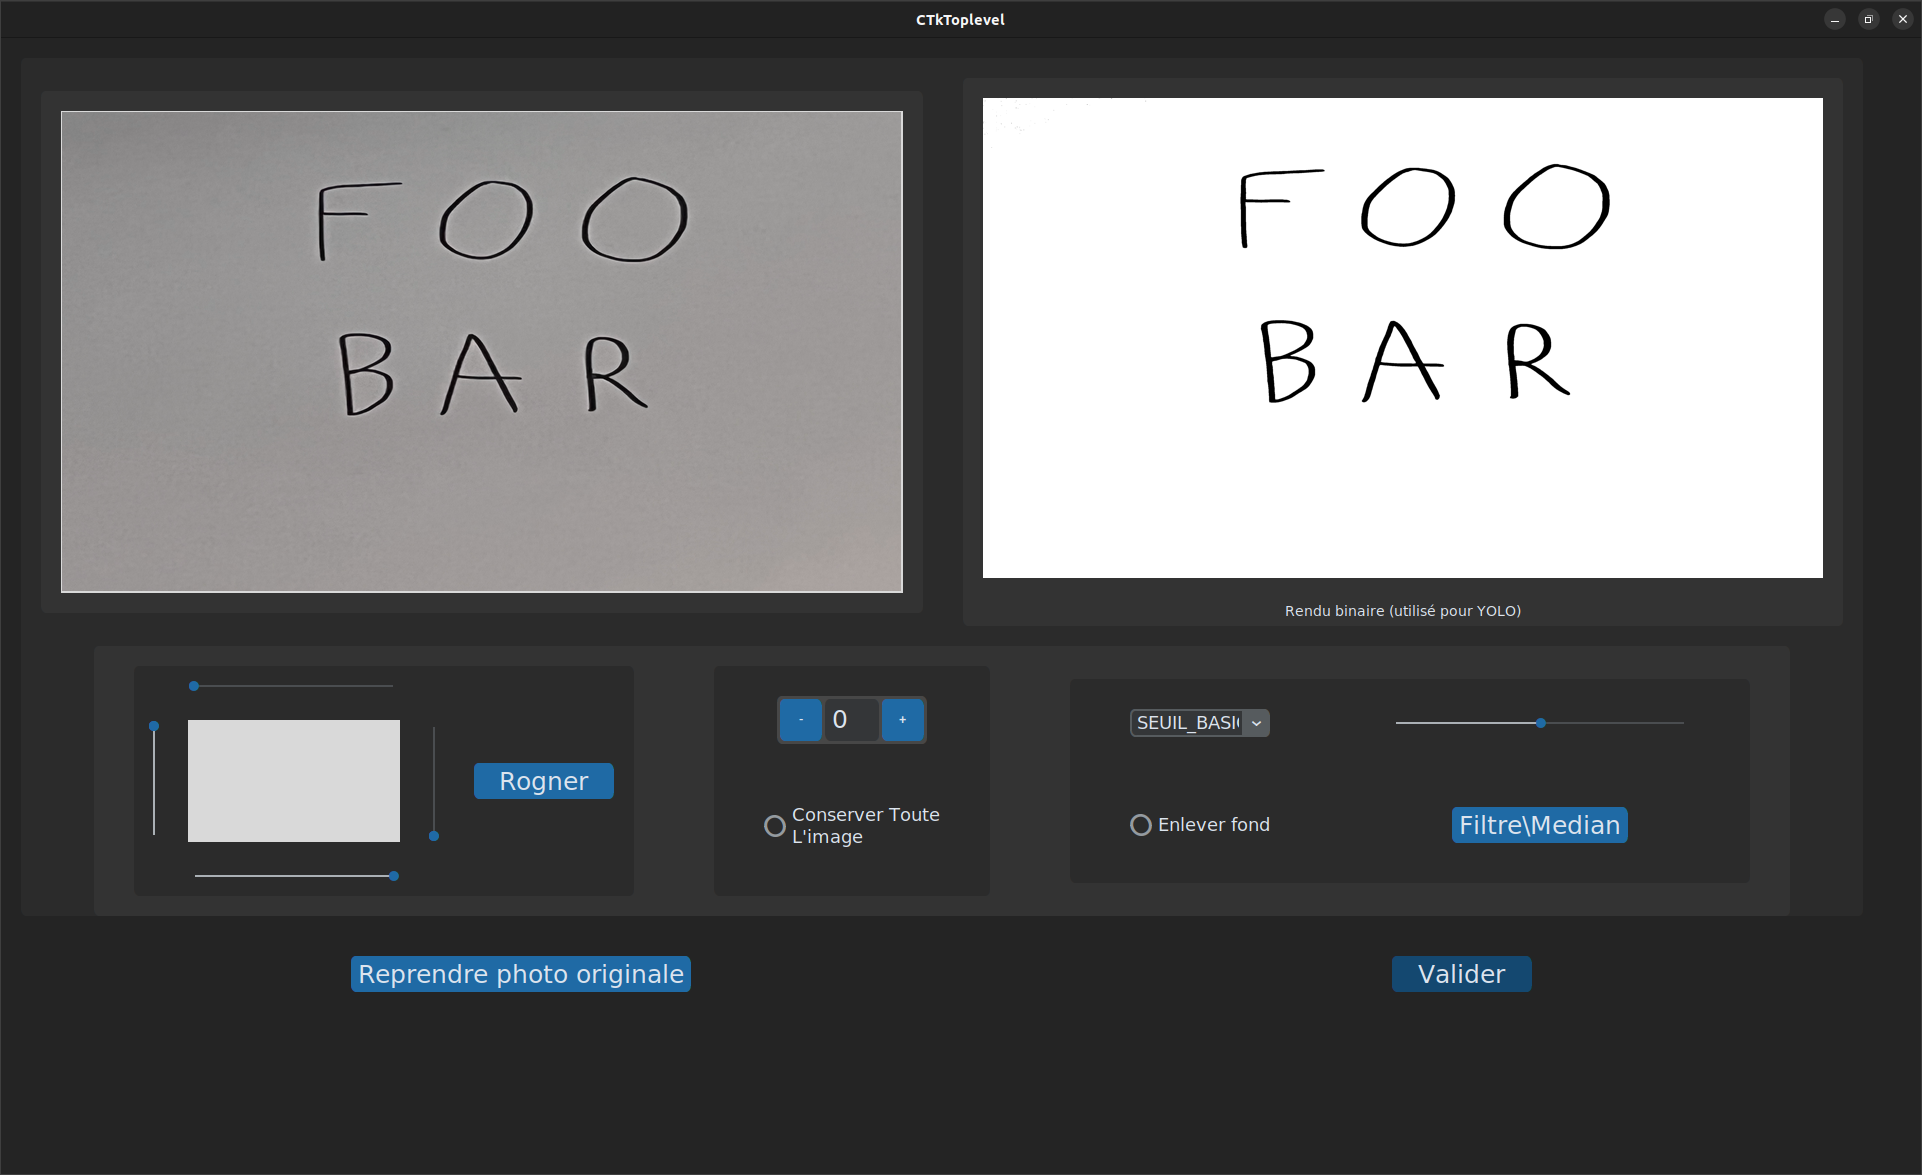
\includegraphics[width=0.8\textwidth]{modif.png}
				\caption{Fenêtre de l'IHM où l'on peut rogner, pivoter et filtrer une image}
				\label{fig:modif}
			\end{figure}
			\paragraph{}
				Après avoir entrer une image (figure 2 A), une étape de préprocessing (découpage) peut-être établi pour réduire le bruit concentrer sur les bords de l'image et causé par la lumière .
				L'image résultat est convertie après en image binaire réalisé avec un seuil adapté. Puis, les pixels noirs et blancs ont été inversé pour facilité la segmentation des images.
				%il est possible qu'il y ait beaucoup de bruit, dans ce cas là, nous pouvons rogner l'image pour enlever des ombres sur les bords, faire des rotations et filtrer pour enlever le bruit comme illustrée sur la figure \ref{fig:modif}
			\begin{figure}[H]
				\centering
				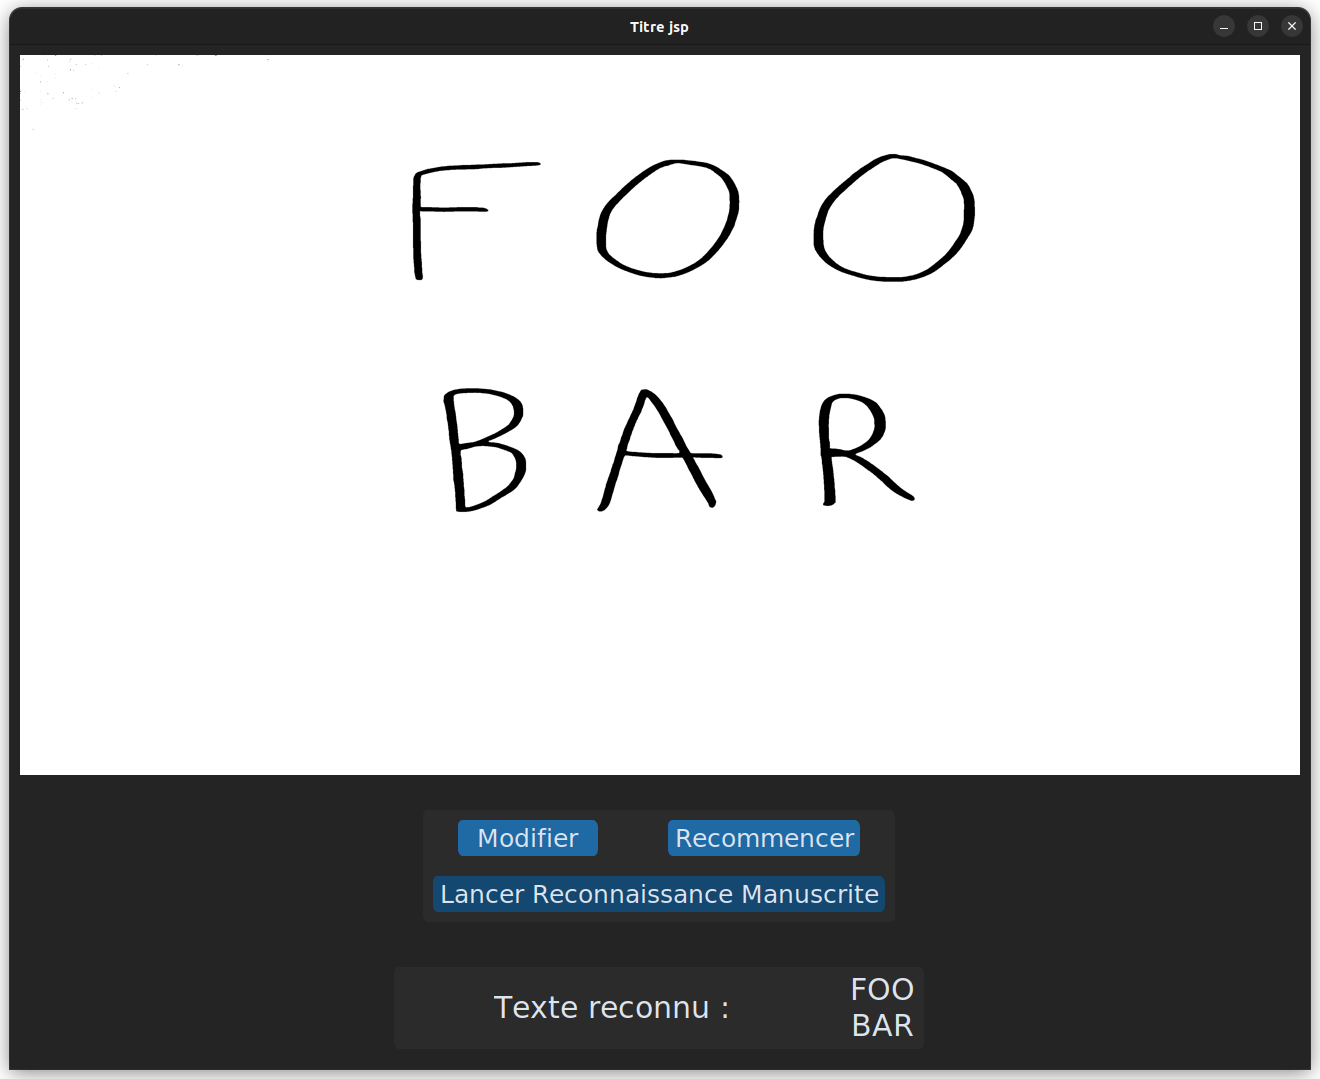
\includegraphics[width=0.8\textwidth]{recon.png}
				\caption{Fenêtre de l'IHM après présentation des caractères reconnus}
				\label{fig:recon}
			\end{figure}

			\paragraph{} Après avoir établi le prétraitement détaillé ci-dessus, une segmentation des caractères est produite. Chaque caractère est ensuite reconnu séparément par YOLO. L'IHM affiche la lettre la plus probable pour chaque objet détecté.
			% \paragraph{} La segmentation des caractères 
			% \paragraph{}Notre programme va segmenter les caractères, en faire des imagettes et donner ces imagettes individuellement à YOLO. Ensuite après cette reconnaissance, l'IHM présente le résultat.


			\subsection{Filtres et seuillage}
			Le pré-traitement de l'image est une phase importante qui affecte le bon déroulement de toutes les étapes futures. Les images prises par les appareils photos souffrent en général de divers problème liés à la difficulté de l'acquisition (manque de luminosité, présence de bruit, éclairage inhomogène, texte penché etc)
			Puisque chaque image comporte des défauts qui lui sont propres, certains seuils et certains filtres seront plus adaptés que d'autres pour obtenir binarisation de qualité.
			
				\subsubsection{Seuillage global}
				
				\paragraph{} Le seuillage global consiste à diviser une image (en niveau de gris), en deux parties en utilisé une valeur prédéfinie appelée “seuil global”. Chaque pixel prend la valeur 0 (noir) si sa valeur initiale est en dessous du seuil global et 255 (blanc) sinon.
				Le seuillage global est une méthode simple qui offre une binarisation sans bruit et qui suffit lorsque l'acquisition est de bonne qualité. (mettre les images)
				
				
				\begin{figure}[h]
					\centering
					\begin{minipage}{.5\textwidth}
					  \centering
					  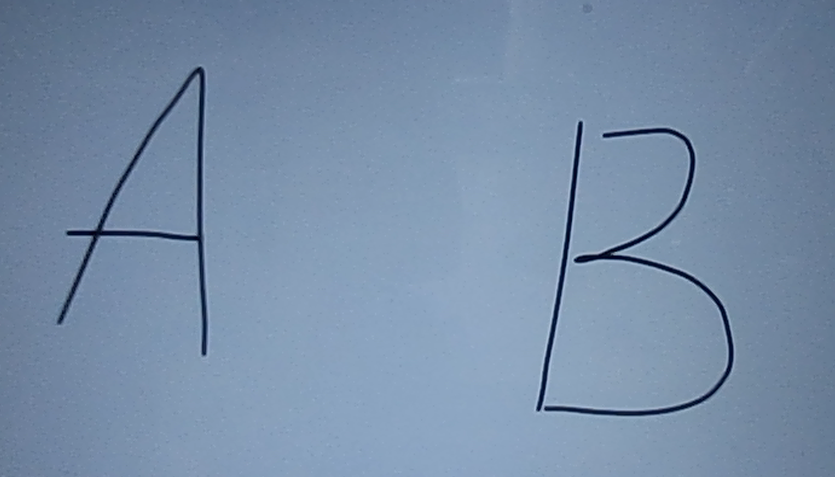
\includegraphics[width=.8\linewidth]{imageSansSeuilBien.png}
					  \caption{image prise par l'appareil photo}
					  \label{fig:imageSansSeuilGlobal}
					\end{minipage}%
					\begin{minipage}{.5\textwidth}
					  \centering
					  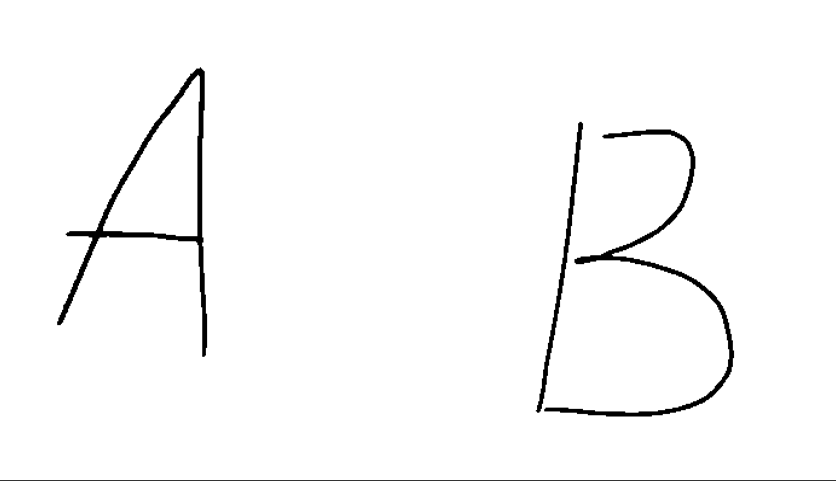
\includegraphics[width=.8\linewidth]{imageSeuilGlobalBien.png}
					  \caption{image après seuillage global }
					  \label{fig:imageSeuilGlobalBien}
					\end{minipage}
				\end{figure}


				\paragraph{} Cependant si l'image souffre d'un éclairage inhomogène le seuillage global devient inefficace. 
				


				\begin{figure}[h]
					\centering
					\begin{minipage}{.5\textwidth}
					  \centering
					  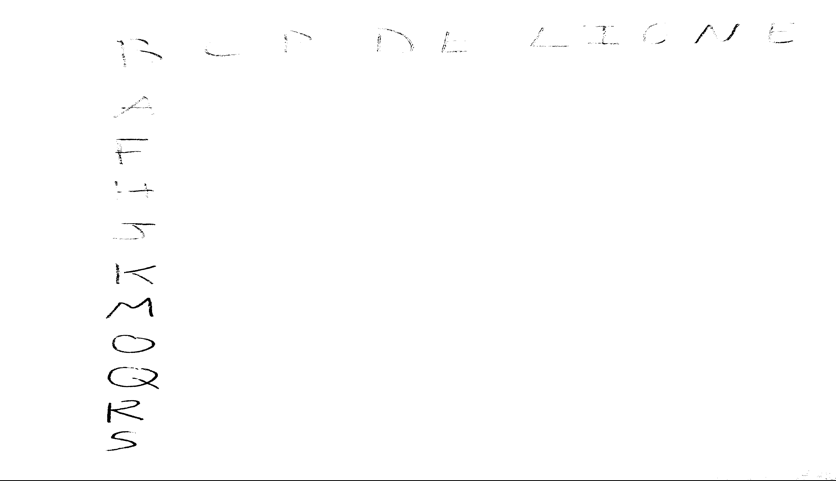
\includegraphics[width=.8\linewidth]{seuil80.png}
					  \caption{Seuillage global à 80}
					  \label{fig:imageSeuilGlobal80}
					\end{minipage}%
					\begin{minipage}{.5\textwidth}
					  \centering
					  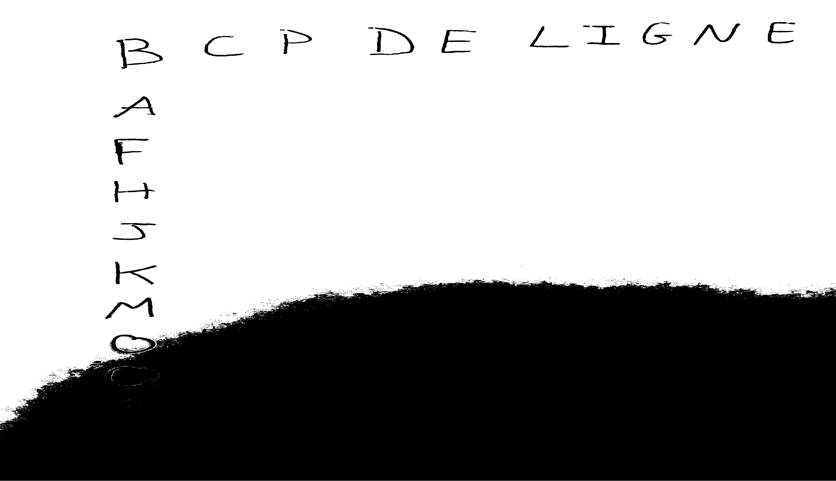
\includegraphics[width=.8\linewidth]{seuil140.png}
					  \caption{Seuillage global à 140 }
					  \label{fig:imageSeuilGlobal140}
					\end{minipage}
				\end{figure}



				\subsubsection{Seuillage adaptatif}
				\paragraph{} Contrairement à la méthode de seuillage global, qui utilise un seuil unique pour diviser une image en deux parties,
				la méthode de seuillage adaptatif utilise un seuil différent pour chaque pixel de l'image en fonction de la valeur de ses voisins. 
				Cela est particulièrement efficace pour exposer les lignes et les contours de l'image, et donc pour exhiber les lettres manuscrites. 
				Il faut noter cependant que la binarisation produite contient du bruit “poivre et sel” (des valeurs anormalement basses ou haute à certains endroits). Pour pallier ce problème, nous appliquons au préalable un filtre médian sur l'image en niveau de gris.
				
				\begin{figure}[h]
					\centering
					\begin{minipage}{.5\textwidth}
					  \centering
					  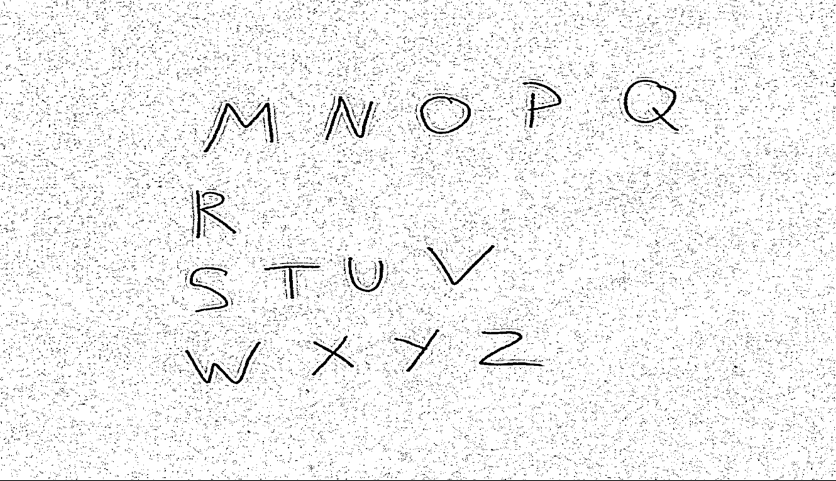
\includegraphics[width=.8\linewidth]{seuilAdaptatif.png}
					  \caption{Seuil adaptatif}
					  \label{fig:seuillageAdaptatif}
					\end{minipage}%
					\begin{minipage}{.5\textwidth}
					  \centering
					  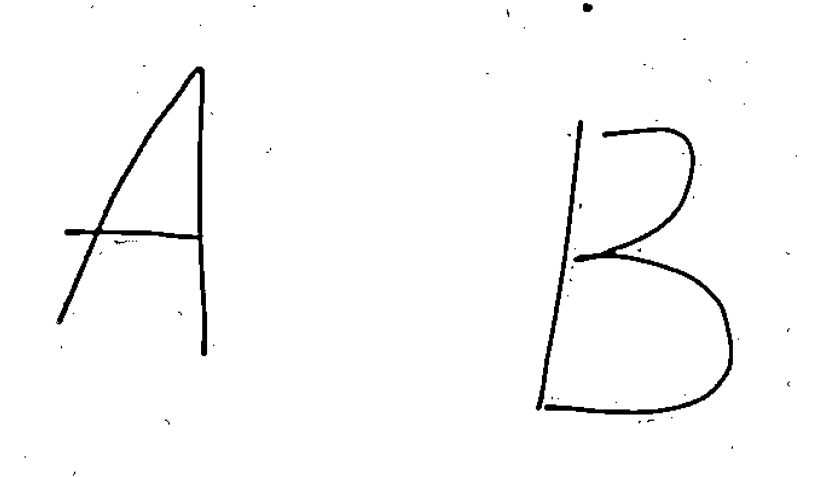
\includegraphics[width=.8\linewidth]{seuilAdaptatifGauss.png}
					  \caption{Seuil adaptatif avec un filtre gaussien}
					  \label{fig:seuillageAdaptatifEtGauss}
					\end{minipage}
				\end{figure}


				

				\subsubsection{Seuillage de Sauvola}
				\paragraph{} La méthode de Sauvola, qui se base également sur un seuillage local, vise à améliorer la qualité de la binarisation en présence d'un éclairage inhomogène et de variations locales de la luminance. Pour chaque pixel, le seuil est déterminé par cette formule mathématique :
							T(x,y) = m(x,y) * (1 + k * (s(x,y) / R - 1))
				où T(x,y) est le seuil pour le pixel à la position (x,y), m(x,y) est la moyenne locale des niveaux de gris, s(x,y) est l'écart type local des niveaux de gris, k est un paramètre de pondération et R est la valeur de l'échelle fixe.
				Cette méthode est particulièrement adaptée pour la segmentation de l'écriture manuscrite à condition de choisir une bonne valeur pour k. 



				\subsubsection{Seuillage Otsu}
				\paragraph{} La méthode d'Otsu effectue simplement un seuillage global, mais en minimisant l'écart entre le nombre de pixels blancs et le nombre de pixels noirs. Pour la reconnaissance de l'écriture manuscrite, il peut être utile pour différencier le support d'écriture (en général une feuille blanche) du reste de la scène.
				Pour exploiter au mieux ce seuil, il faut d'abord appliquer un flou gaussien qui égalise la couleur du support d'écriture (supposée uniforme). 
				Il se peut que le seuillage identifie les lettres comme élément du second plan. Dans ce cas, nous effectuons une fermeture (une dilatation suivie d'une érosion) sur l'image seuillée.
				

				\begin{figure}[h]
					\centering
					\begin{minipage}{.5\textwidth}
					  \centering
					  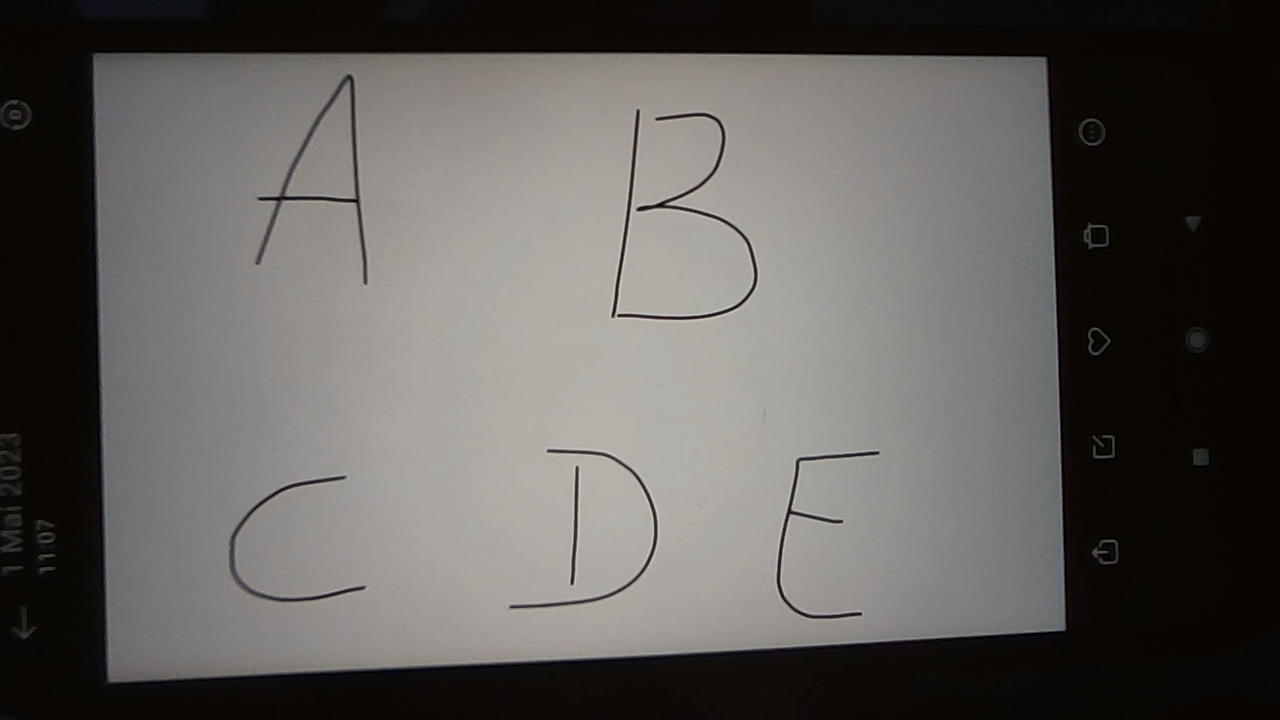
\includegraphics[width=.8\linewidth]{sansOtsu.png}
					  \caption{image de base}
					  \label{fig:sansOtsu}
					\end{minipage}%
					\begin{minipage}{.5\textwidth}
					  \centering
					  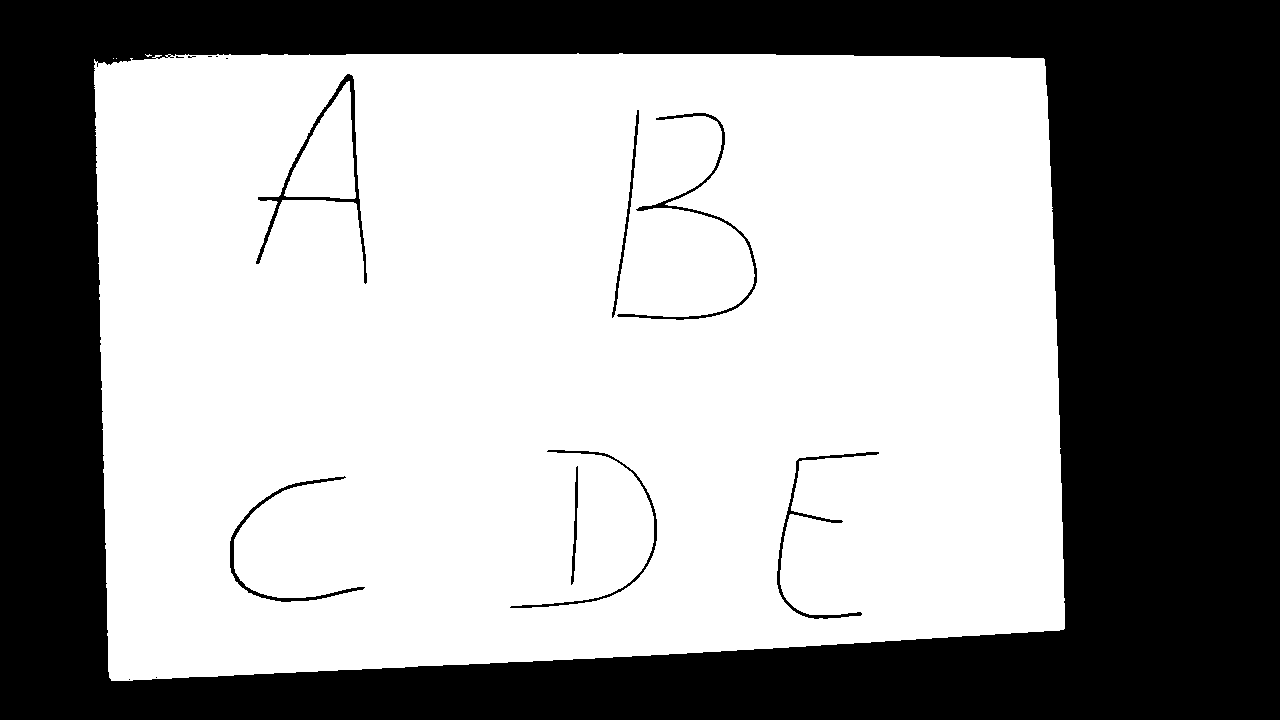
\includegraphics[width=.8\linewidth]{apresOtsu.png}
					  \caption{après seuil otsu}
					  \label{fig:apresOtsu}
					\end{minipage}
				\end{figure}


				\begin{figure}[h]
					\centering
					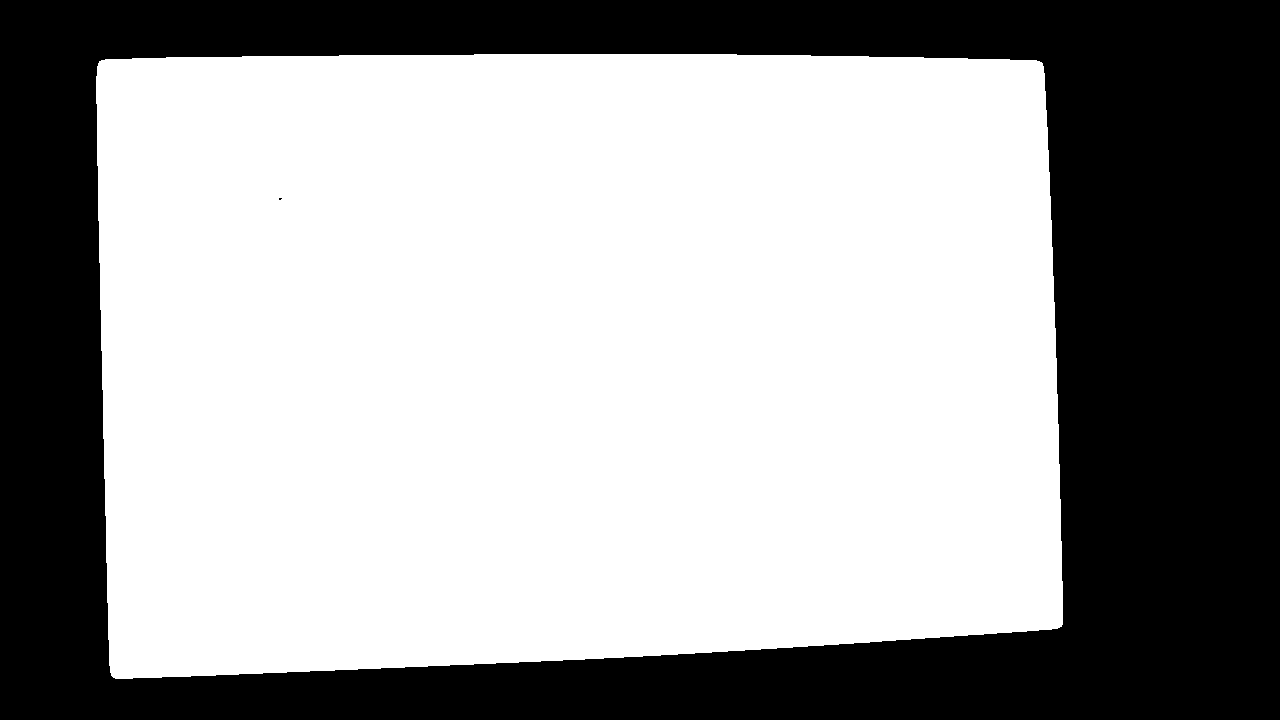
\includegraphics[width=0.4\textwidth]{apresFermeture.png}
					\caption{apres la fermeture}
					\label{fig:apresFermeture}
				\end{figure}

				\paragraph{} Après avoir obtenu la position de la feuille, nous appliquons un NON binaire pour nous en servir comme masque. Après un OU binaire entre ce masque et l'image d'origine, le texte apparait sans la scène (mal dit à reformuler)



				\begin{figure}[h]
					\centering
					\begin{minipage}{.5\textwidth}
					  \centering
					  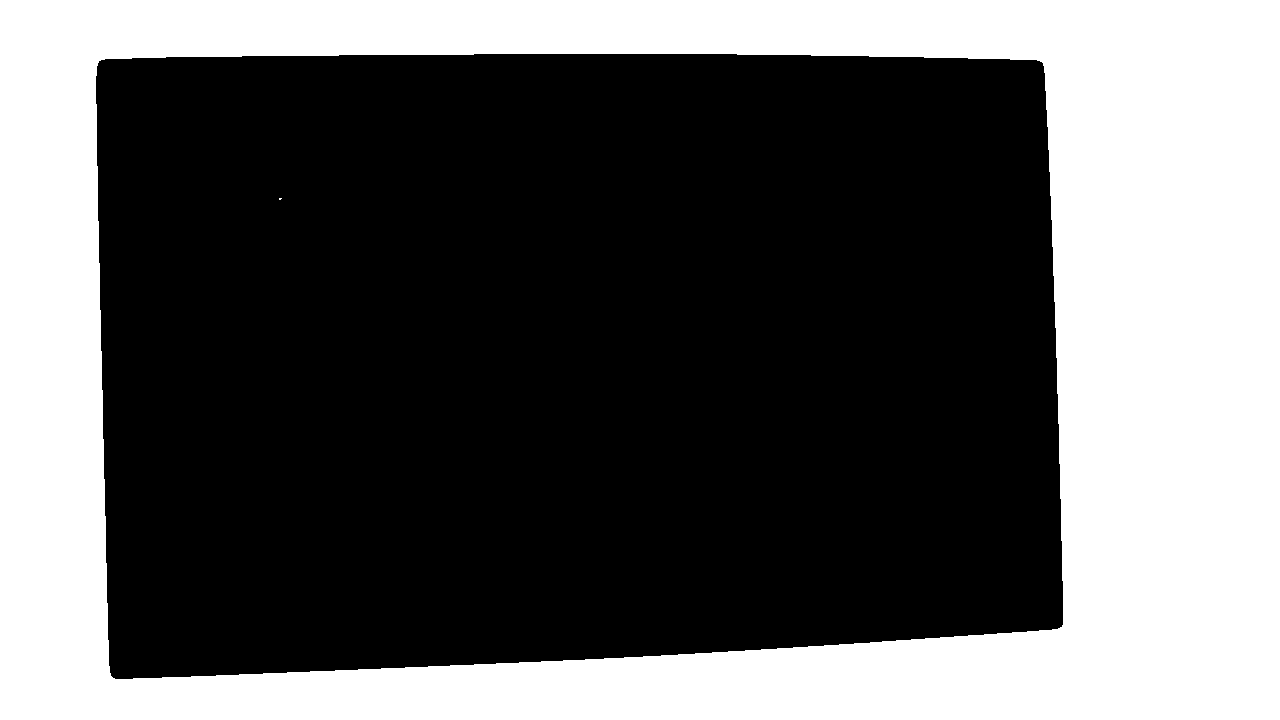
\includegraphics[width=.8\linewidth]{nonBinaireOtsu.png}
					  \caption{NON binaire}
					  \label{fig:nonBinaireOtsu}
					\end{minipage}%
					\begin{minipage}{.5\textwidth}
					  \centering
					  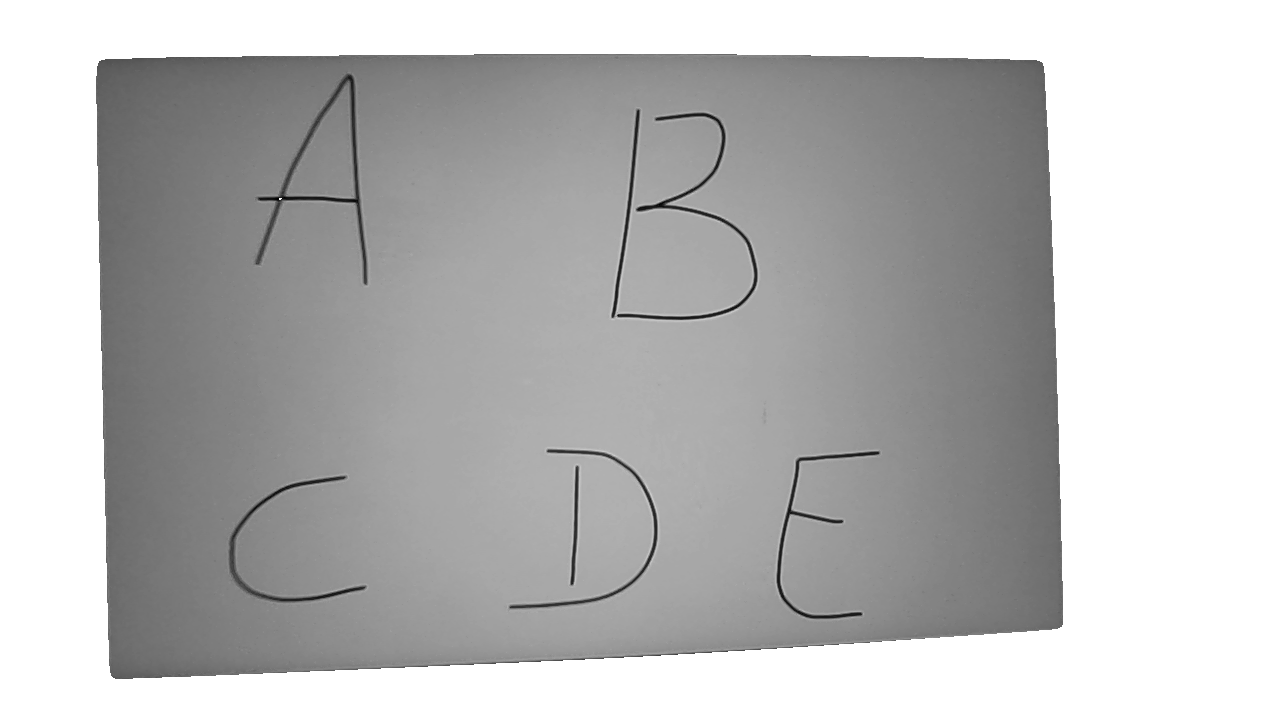
\includegraphics[width=.8\linewidth]{imageSansFond.png}
					  \caption{image Sans le fond}
					  \label{fig:imageSansFond}
					\end{minipage}
				\end{figure}


				




			

			\subsection{Segmentation} 
				\paragraph{} Une fois l'image binarisée, il faut maintenant séparer chaque caractère présent dans l'image.
				
				\paragraph{} Dans un premier temps, une projection horizontale de histogramme de l'image binaire est calculée afin de segmenter les lignes de texte présentes dessus; 
				\paragraph{} cette projection de l'histogramme correspond à un vecteur de taille égale à la largeur de l'image et sommant le nombre de pixels noirs sur une ligne. % Par la suite, nous avons écrit une fonction pour créer une image pour l'histogramme précédent.
				Les images d'entrée ne sont pas toujours parfaites, ce qui provoque l'apparition d'anomalies dans la projection, pouvant ainsi fausser l'analyse de l'image. Face à ce problème, nous avons créé des fonctions permettant de reconnaître et de supprimer ces anomalies que ce soit pour la segmentation des lignes ou des caractères.
				Après la segmentation des lignes et en se basant sur l'analyse de la projection verticale de l'histogramme de celles-ci, nous avons implémenté des fonctions permettant la localisation et la segmentation des caractères présents dans les lignes. 
				Le critère de détection est basé sur la succession de projections nulles et non nulles. En sortie, nous optenons l'image de chaque caractère et de chaque ligne.
				(faudrait dire "voir algo en référençant la bonne page)
			% relire et reformuler
			
			% \paragraph{}Il est possible de voir les imagettes générées dans le dossier "./images/imageSegmentee"
		
		


		\subsection{Entrainement de YOLO}

			\paragraph{} Pour prédire et classer au mieux les caractères segmentés produits, les réseaux de neurones ont besoin d'une première phase d'entrainement à partir d'un grand nombre de données.
			Concernant les images d'entrainement, nous avons choisi la base de données d'images d'écriture manuscrite développée par le National Institute of Standards and Technology (NIST).
			Cette base de données contient des images de caractères manuscrits et de formulaires remplis à la main, qui ont été collectées pour soutenir la recherche en reconnaissance d'écriture manuscrite.
			
			\begin{figure}[h]
				\centering
				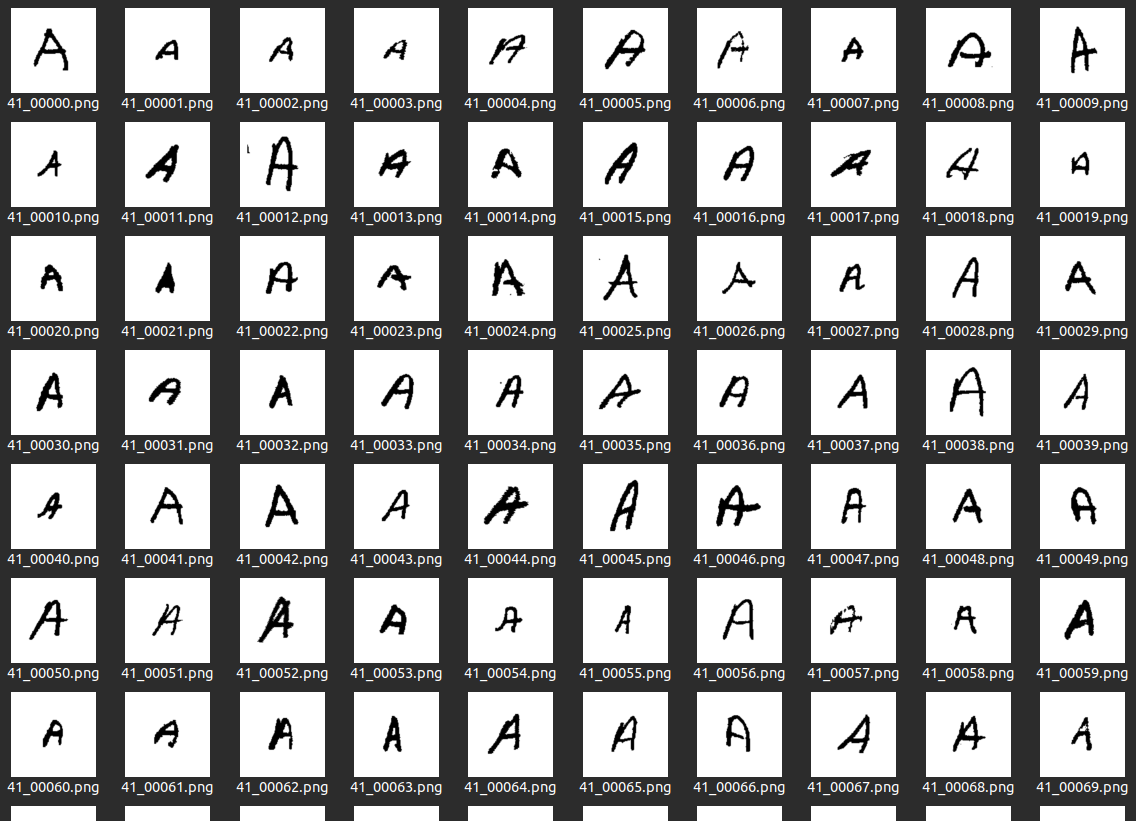
\includegraphics[width=0.6\textwidth]{lettreABDD.png}
				\caption{Un exemple pour la lettre A}
				\label{fig:BDDNIST}
			\end{figure}
		
			\paragraph{} Cette banque d'image contient en tout 800 000 caractères, écrits par 3600 personnes différentes. Avant d'entrainer notre réseau de neurones,
			il faut conformer ces images aux images produite par notre segmentation. Nous avons donc enlever les bords blancs de chaque image de la banque d'image et redimensionner en 128x128.


			\begin{figure}[h]
				\centering
				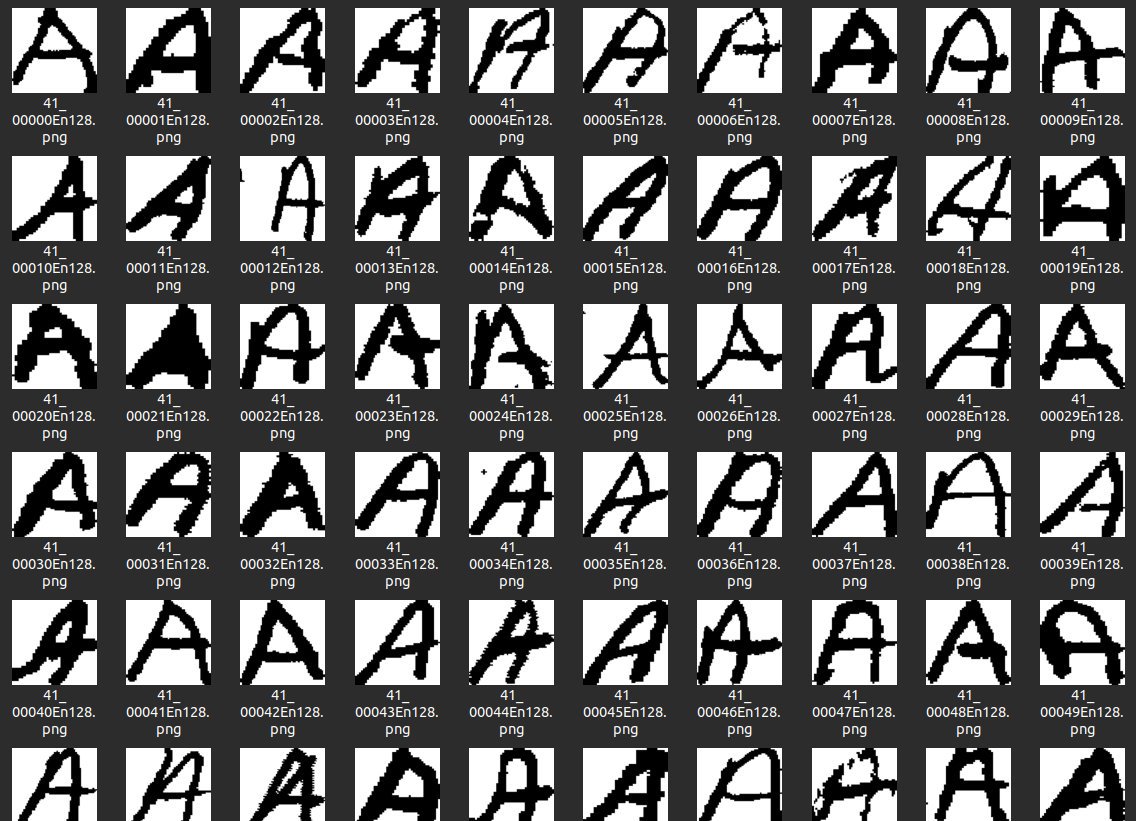
\includegraphics[width=0.6\textwidth]{lettreASansBordBDD.png}
				\caption{lettre A après découpage et redimension}
				\label{fig:BDDNISTsansBord}
			\end{figure}

			\paragraph{} Une fois le set de données préparé, nous pouvons passer à l'apprentissage.
			Nous pouvons paramétrer l'entraînement dans YOLO à l'aide des "hyperparamètres", qui ne sont pas des paramètres appris à partir des données, mais plutôt définis par l'utilisateur avant l'entraînement du réseau. Ils contrôlent divers aspects de l'apprentissage et peuvent affecter considérablement les performances du réseau.
			Il est important de modifier et de tester des paramètres différents lorsque les résultats ne sont pas suffisament acceptables.
			Etant donné que nos images sont assez petites et binarisées et que nos objets sont assez faciles à reconnaitre, les paramètres par défaut de YOLO nous suffisent à avoir des résultats convenables.



			\subsection{Statistiques}
			\begin{itemize}
				\item[•] Nombres de lignes de code : 
				\item[•] Nombres de script
			\end{itemize}
	
	\newpage

	
	\section{Algorithmes et Analyse}
		% \subsection{YOLO}
		\subsection{Segmentation par histogramme de projection}
			\begin{algorithm}

				\SetKwInput{Strat}{Stratégie}
				\LinesNumbered
				\caption{SEGMENTATION(image)}\label{alg:segmentation}
				\KwData{image en RGB}
				% \KwOut{output}
				% \KwOut{output}
				\Strat{la segmentation se produit en deux temps. 
				En premier, la segmentation des lignes avec la projection verticale, 
				et par la suite la segmentation des caractères par la projection horizontale.}
				\KwResult{\\Tableau de couples d'entier représentant les coordonnées en y de début et de fin des n des lignes sur l'image.
        				\\Tableau de tableau de couple d'entier représentant les coordonnées en x de début et de fin des n lettres contenues dans chaque ligne.
        				\\Tableau d'image des lignes
						\\Tableau de tableau d'image des caractères}
				\BlankLine
				$ndgImage \gets convertirImageEnNDG(image)$\;
				\BlankLine
				\tcc{on met l'image en noir et blanc sauf que le seuillage est inversé}
				$imageBinaire \gets binarisationInversé(ndgImage)$\;
				\BlankLine
				\tcc{on fait la somme des pixels sur les colonnes et on les divise par 255}
				$projectionHorizontale = (sommeValPixel(imageBinaire, axe=1)) / 255$\;
				$delimitationDesLignes = coordonneeLigne(projectionHorizontal)$\;
				\BlankLine
				$imagesLignes = []$\;
				\BlankLine
				\tcc{on copie une zone de l'image correspondant à une ligne grâce aux coordonnées calculées\\et on l'ajoute à notre tableau d'image de lignes}
				\For{(x,y) dans delimitationDesLignes}{imagesLignes.ajouter(ndgImage[x:y, 0:longeurImage])}
				\BlankLine
				\tcc{on initialise le tableau de tableaux des images de Caractère on fonction du nombre de ligne detecté}
				$imagesCaracteres = [[ ] pour i allant de 0 à longeur(imagesLignes)]$\;
				\BlankLine
				\tcc{on initialise le tableau de tableaux de couple de coordonnées  on fonction du nombre de ligne}
				$coordonneesCaracteres = [[] pour i allant de 0 à longeur(imagesLignes)]$\;
				\BlankLine
				\For(){index, uneLigne dans imagesLignes}
				{
					$ligneBinaire = binarisationInversé(uneLigne)$\;
					\tcc{on fait la somme des pixels sur les lignes de l'image et on les divise par 255}
					$projectionVerticale = (sommeValPixel(imageBinaire, axe=0)) / 255$\;
					$delimitationDesCaracteres = coordonneeCaractere(projectionVerticale)$\;
					\BlankLine
					\tcc{on ajoute les coordonnées au tableau de coordonnées}
					$coordonneeCaractere[index].ajouter(delimitationDesCaracteres)$\;
					\tcc{on copie une zone de l'image correspondant à un caractère grâce aux coordonnées calculées\\et on l'ajoute à notre tableau d'image de caractère}
    				\For(){(x,y) dans delimitationDesCaracteres}
					{
						$imagesCaracteres[index].ajouter(ndgImage[0:hauteurUneLigne, x:y])$\;
					}
					$redimensionnerImage(binarisation(imagesCaracteres[index],hauteur = 128,longeur = 128), seuil = 127)$\;
					\BlankLine
				}
				\KwRet{$delimitationDesLignes,delimitationDesCaracteres,imagesLignes,imagesCaracteres$}
			\end{algorithm}
			\newpage
			\begin{algorithm}
				\SetKwInput{Strat}{Stratégie}
				\LinesNumbered
				\caption{COORDONNEECARACTERE(T)}\label{alg:coordcar}
				\KwData{tableau de flottant représentant la projection vertical d'une image}
				\Strat{Trouver les zones non nul dans l'histogramme}
				\KwResult{tableau de couple d'entier indiquant les coordonnées du début et de la fin d'une lettre}
				\BlankLine
				$coordCaractere = []$\;
				\BlankLine
				$dansLeCaractere = False$\;
				\tcc{Début = pair	Fin = impair}
				$DF = []$\;
				\BlankLine
				\For{i de 0 à taille(T)}
				{
					\If{$T[i] \neq 0$}{
						\If{!dansLeCaractere \textbf{or} (dansLeCaractere  \textbf{and} i == taille(T)-1)} {
							$DF.ajouter(i)$\;
							\If{i == taille(myprojection)-1 et taille(DF) mod 2 != 0} {
								$supprimer(DF[taille(DF)-1])$\;
							}
						}
						if i == len(myprojection)-1 and len(coordDF)%2!=0:
                    coordDF.pop(-1)
						$dansLeCaractere = True$\;
					}
					\Else{
						\If{dansLeCaractere} {
							DF.ajouter(i)
						}
						$dansLeCaractere = False$\;
					}
				}
				lettres $\gets$ [ (DF[i],DF[i+1]) pour i de 0 à taille(DF) avec un pas de 2 ]\;
				\BlankLine
				\If{taille(lettres)>1}
				{
					$tailleEspacesEntrelettres = [ lettres[i+1][0]-lettres[i][1] pour i de 0 à taille(lettres)-1 ]$\;
					$poidsEspace = trillageCroissant(tailleEspacesEntrelettres)$\;
					\BlankLine
					$SommeIndice \gets 0$\;
					\For{i de 0 à taille(poidsEspace)-1}
					{
						$poidsEspace[i] \gets poidsEspace[i] * (taille(poidsEspace)-i)$\;
						$SI \gets SI + i$\;
					}
					$moyenneEspaces \gets somme(poidsEspace) / SI$\;
					$j \gets 0$\;
					\While{tailleEspacesEntrelettres != []}
					{
						\If{$tailleEspacesEntrelettres < moyenneEspaces*0.2$} {
							$D = lettres[j];$ $supprimer(lettres[j])$\;
							$F = lettres[j];$ $supprimer(lettres[j]);$\;
							\tcc{inserer(tableau, indice, élément)}
							$inserer(lettres,j,(D[0],F[1]))$\;
						}	\lElse{$j \gets j+1$}
						$supprimer(tailleEspacesEntrelettres[0])$\;
					}
				}
				\KwRet{lettres}
			\end{algorithm}
			\begin{figure}
				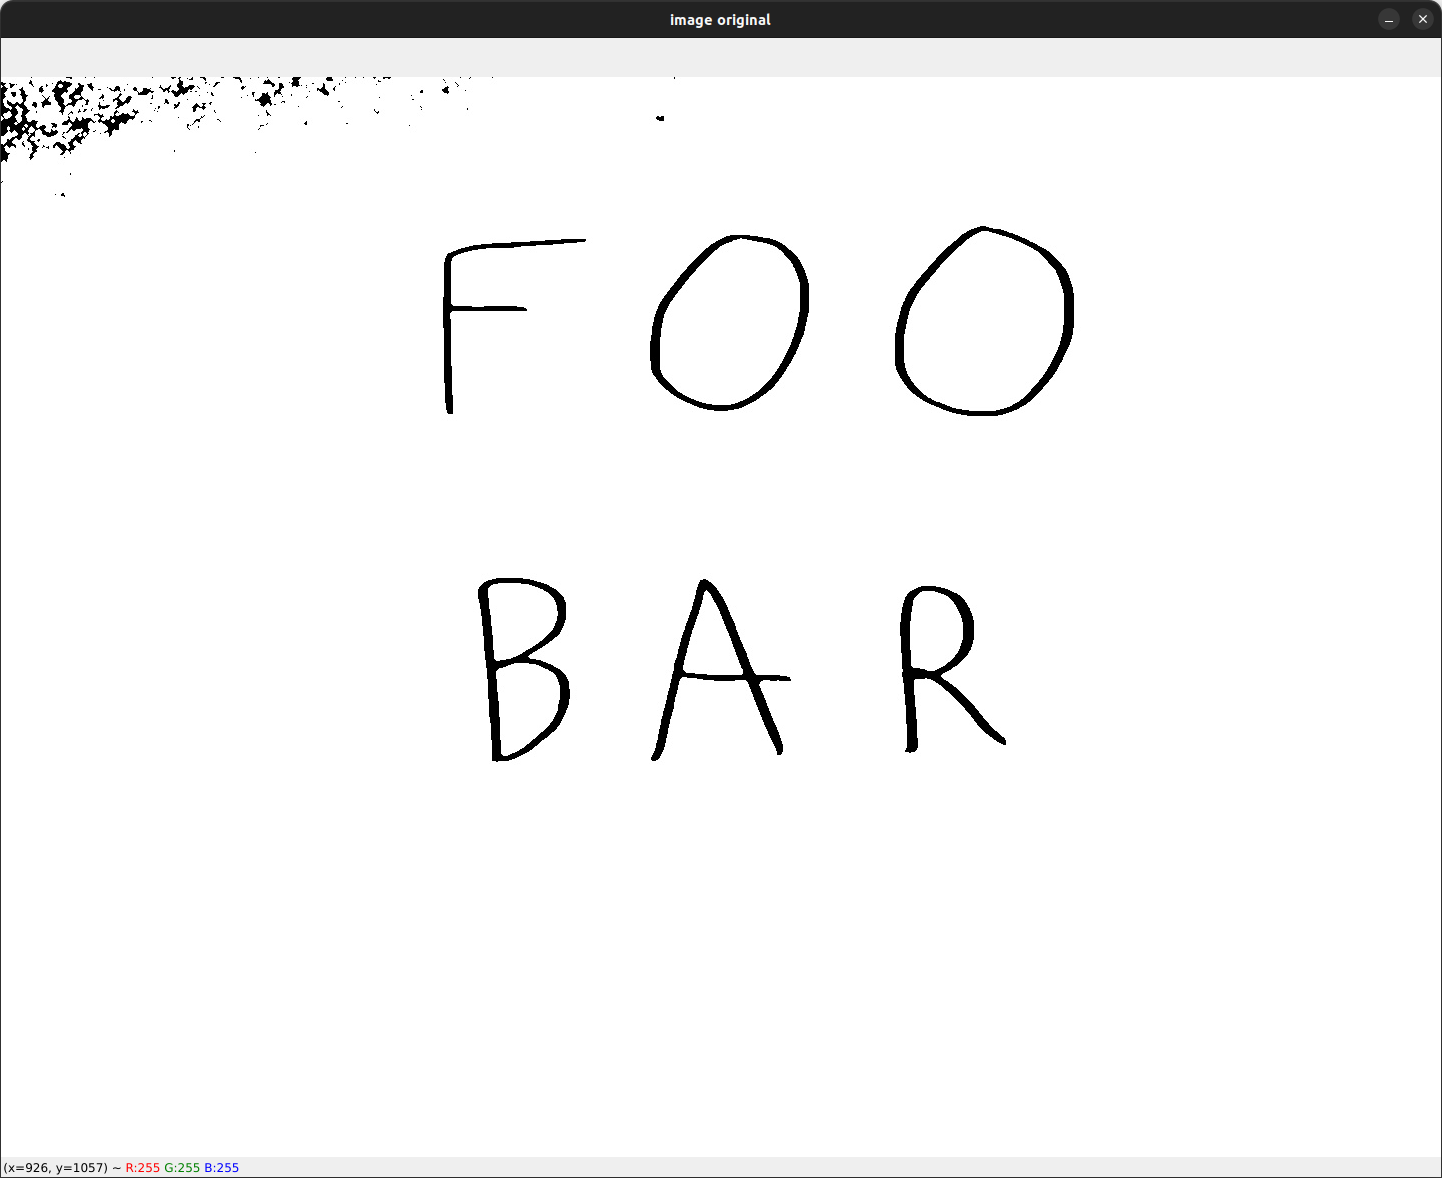
\includegraphics[width=.75\textwidth]{segmentation_image_originel.png}
				\caption{Exemple d'une image après filtrage}
				\centering
				\label{fig:imageOriginel}
			\end{figure}
			\paragraph{} Sur la figure \ref{fig:imageOriginel}, nous voyons une image de bonne qualité prête à être segmenter par l'algorithme n°\ref{alg:segmentation} (page \pageref{alg:segmentation}). 
			\begin{figure}
				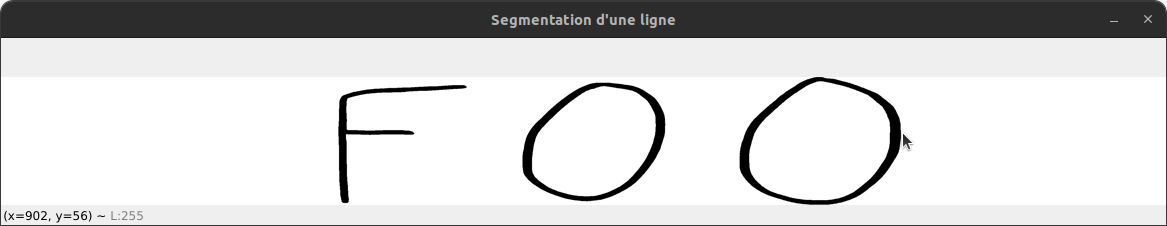
\includegraphics[width=.8\textwidth]{segmentation_ligne1.png}
				\caption{Images de nos 2 lignes créées à partir de l'image de départ}
				\centering
				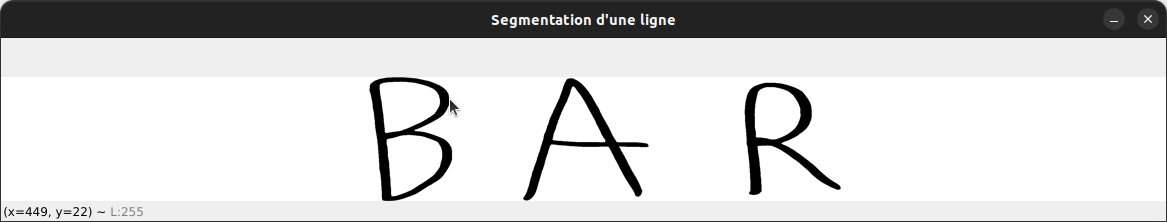
\includegraphics[width=.8\textwidth]{segmentation_ligne2.png}
				\centering
				\label{fig:imageLignes}
			\end{figure}
			% \paragraph{} On voit sur la figure \ref{fig:imageLignes} à la page \pageref{fig:imageLignes} que dû à un filtrage de bonne qualité, nous obtenons exactement 2 lignes comme attendus. 
			\begin{wrapfigure}{r}{0.35\textwidth}
				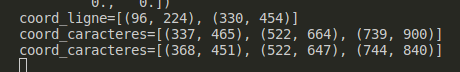
\includegraphics[width=0.35\textwidth]{structDonnee.png}
				\caption{Structure de données dans l'algorithme SEGMENTATION}
					\label{fig:structDonnee}
			\end{wrapfigure}
			\paragraph{} Grâce à une projection vertical, nous obtenons ce tableau (voir figure \ref{fig:structDonnee}). La 1er ligne de ce tableau contient autant de tuples que le nombre de lignes. Chaque tuples contient la composante en ordonnée du début et de la fin d'une ligne. En choississant arbitrairement comme largeur d'une ligne, la largeur de l'image, on extrait nos 2 lignes comme sur la figure \ref{fig:imageLignes}.
			\paragraph{} Maintenant que nous avons isoler les lignes, nous allons maintenant découper les lettres de chaque lignes en suivant l'algorithme n°\ref{alg:coordcar} page \pageref{alg:coordcar}
			\paragraph{} Étant donnée que l'image est filtré, en noir et blanc et binairisé, lorsqu'une lettre est présente à un endroit donnée, cela signifie que sur la projection vertical, l'histogramme est supérieur à 0 à cet endroit là. Sinon, il n'y a pas de lettre et l'histogramme est à 0. L'algorithme n°\ref{alg:coordcar} va parcourir totalement l'histogramme de projection et va tenté de dectecter les pics et récupérer l'indice de début et de fin de ces zones qui correspondront à la limite gauche et droit de la lettre sur l'image. Nous pouvons voir le résultats de cette fonction sur la figure \ref{fig:structDonnee} et des histogrammes de projection horizontal dans l'annexe (page \pageref{fig:histoX1}).
			\begin{figure}
				\caption{Imagettes des caractères crée à partir de la 1e ligne}
				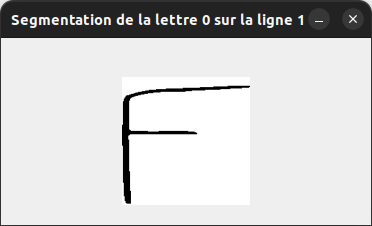
\includegraphics[scale=.3]{segmentation_F.png}
				\centering
				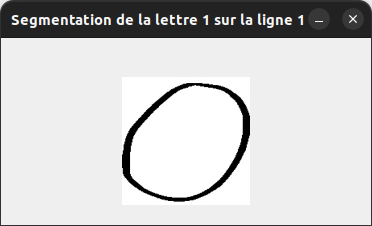
\includegraphics[scale=.3]{segmentation_O1.png}
				\centering
				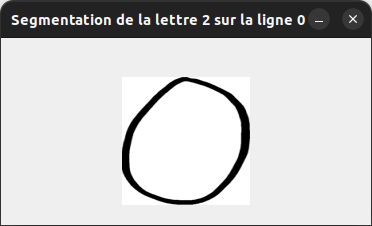
\includegraphics[scale=.3]{segmentation_O2.png}
				\centering
			\end{figure}
			\begin{figure}
				\caption{Imagettes des caractères crée à partir de la 2e ligne}
				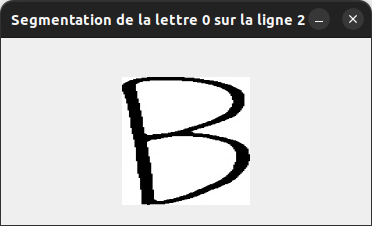
\includegraphics[scale=.3]{segmentation_B.png}
				\centering
				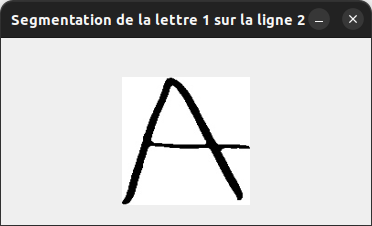
\includegraphics[scale=.3]{segmentation_A.png}
				\centering
				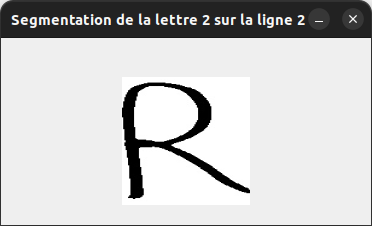
\includegraphics[scale=.3]{segmentation_R.png}
				\centering
			\end{figure}
	\newpage
	\section{Analyse des Résulats}
		\subsection{Mesure expérimental de YOLO}
			\paragraph{} Pour mesurer le taux de prédiction correcte de YOLO, nous avons écrit des lettres de différentes manières et nous avons observer le taux de réussite
			\begin{figure}[H]
				\caption{}
				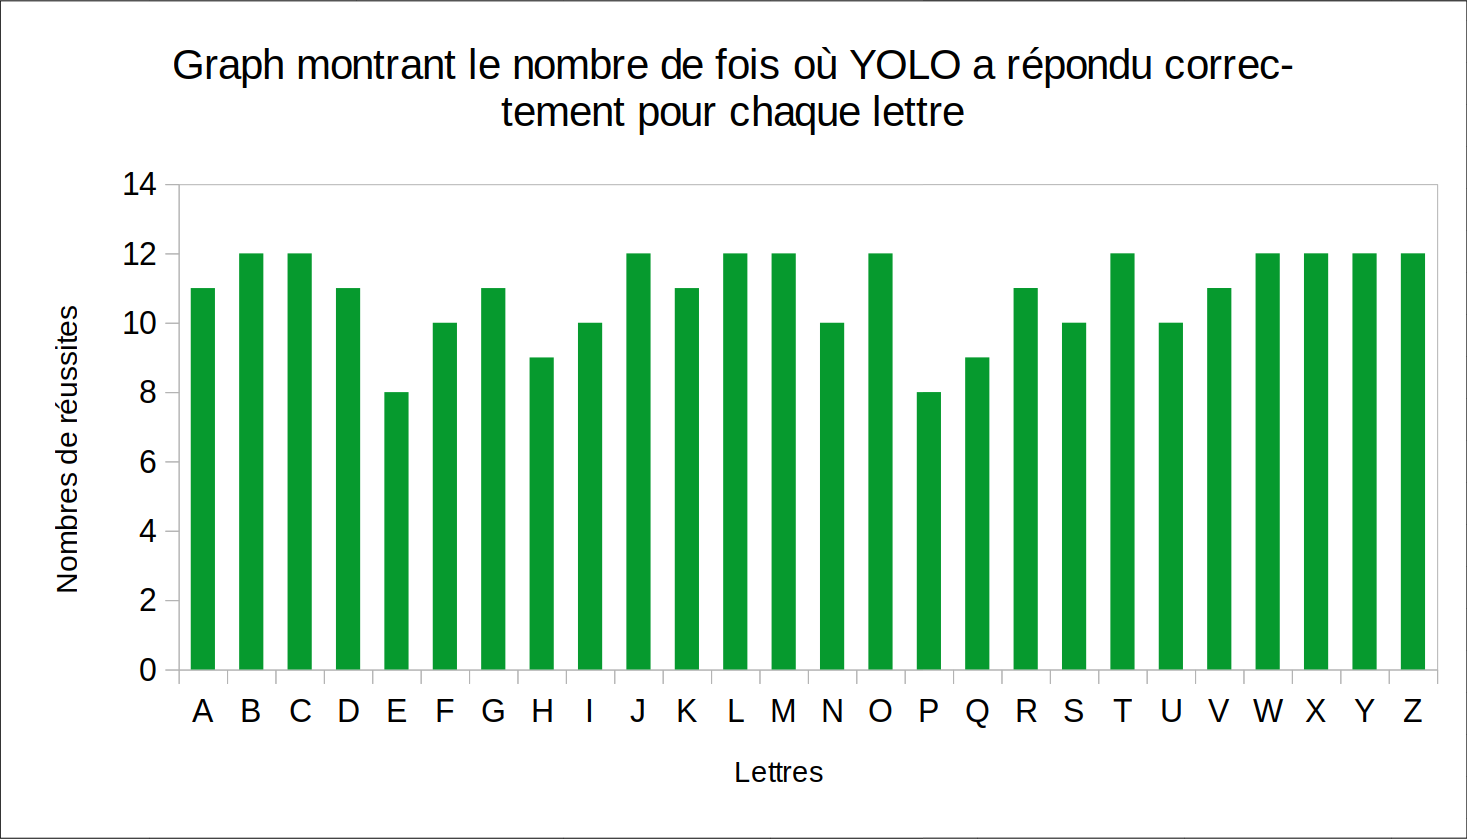
\includegraphics[width=\textwidth]{grapYoloReussite.png}
				\centering
				\label{fig:graph:reussite}
			\end{figure}
			\begin{figure}[H]
				\caption{}
				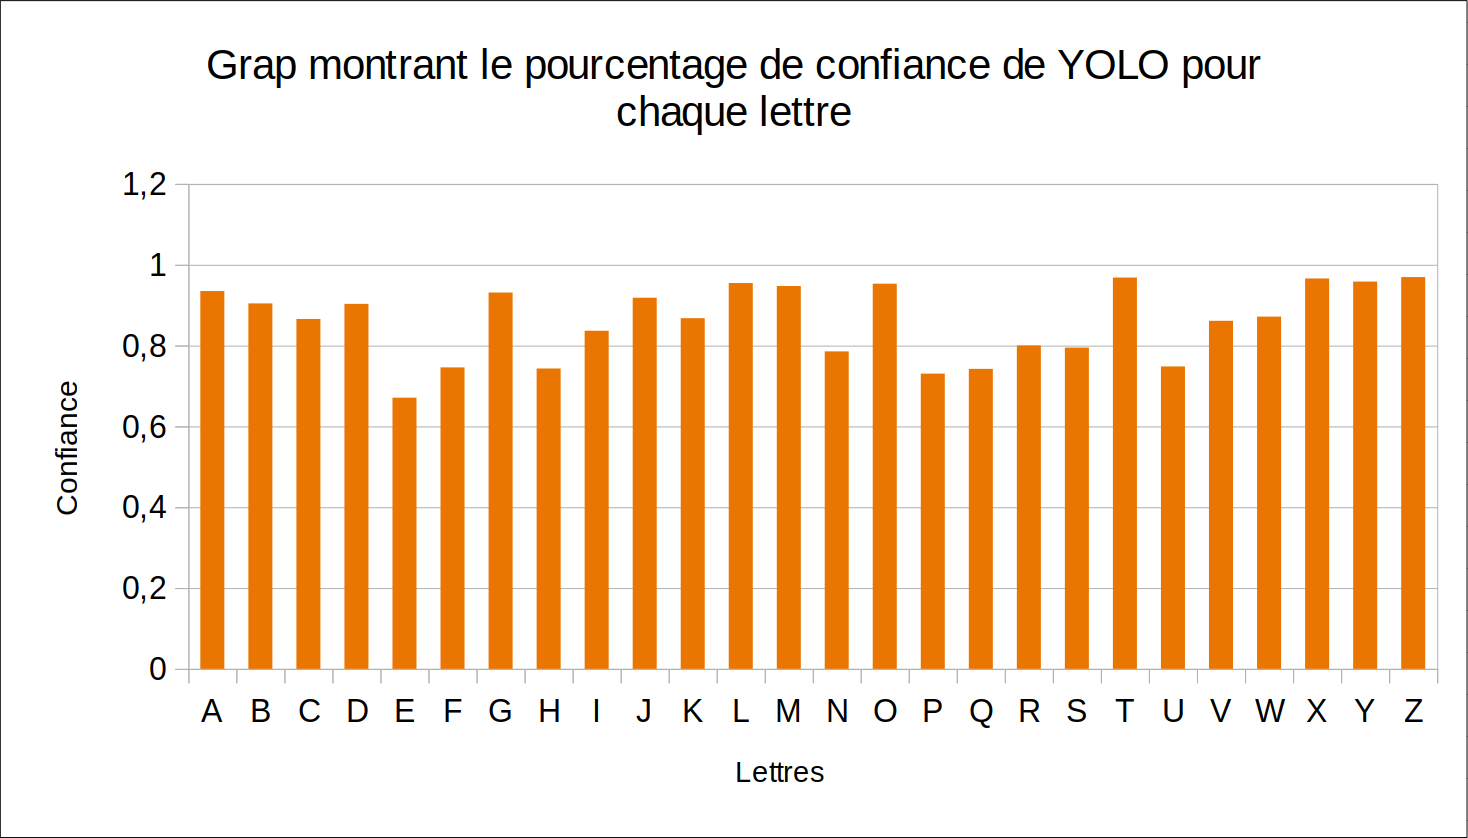
\includegraphics[width=\textwidth]{grapYoloConfiance.png}
				\centering
				\label{fig:graph:confiance}
			\end{figure}
			\paragraph{} YOLO est en général très confiant et arrive dans la plupart des cas à reconnaitre la bonne lettre (dans de bonnes conditions).
		
			\paragraph{} Nous avons utilisé des pangrammes (phrases contenant toutes les lettres de l'alphabet) pour tester notre logiciel.
			
			\begin{center}
				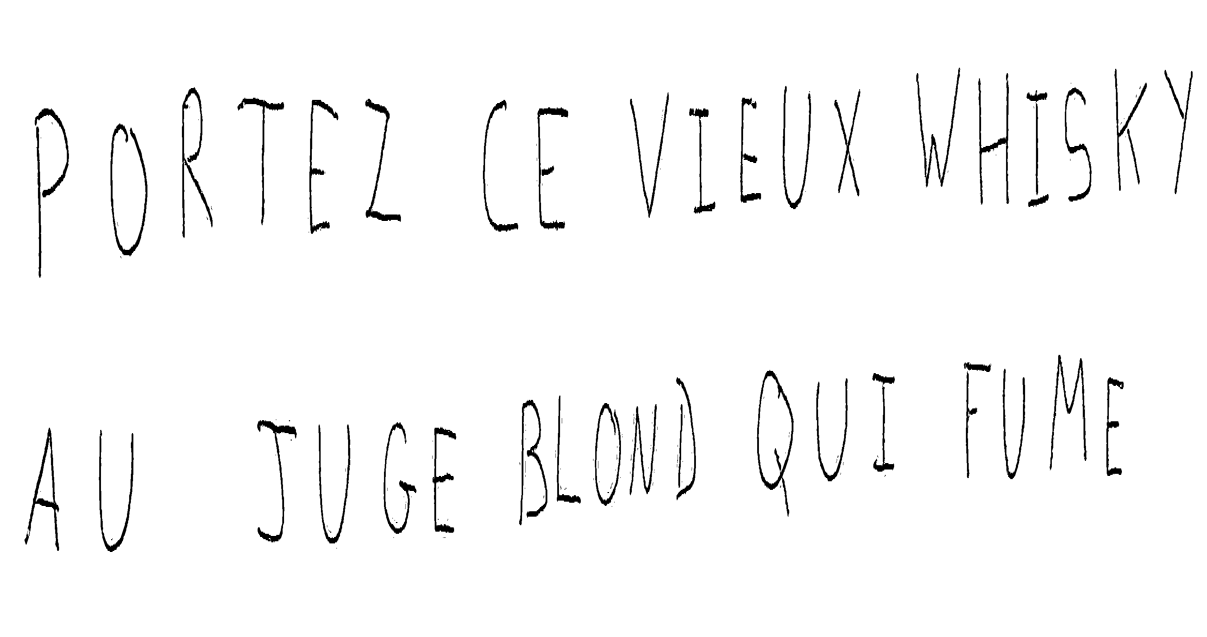
\includegraphics[width=.45\textwidth]{portezCeWhisky.png}
				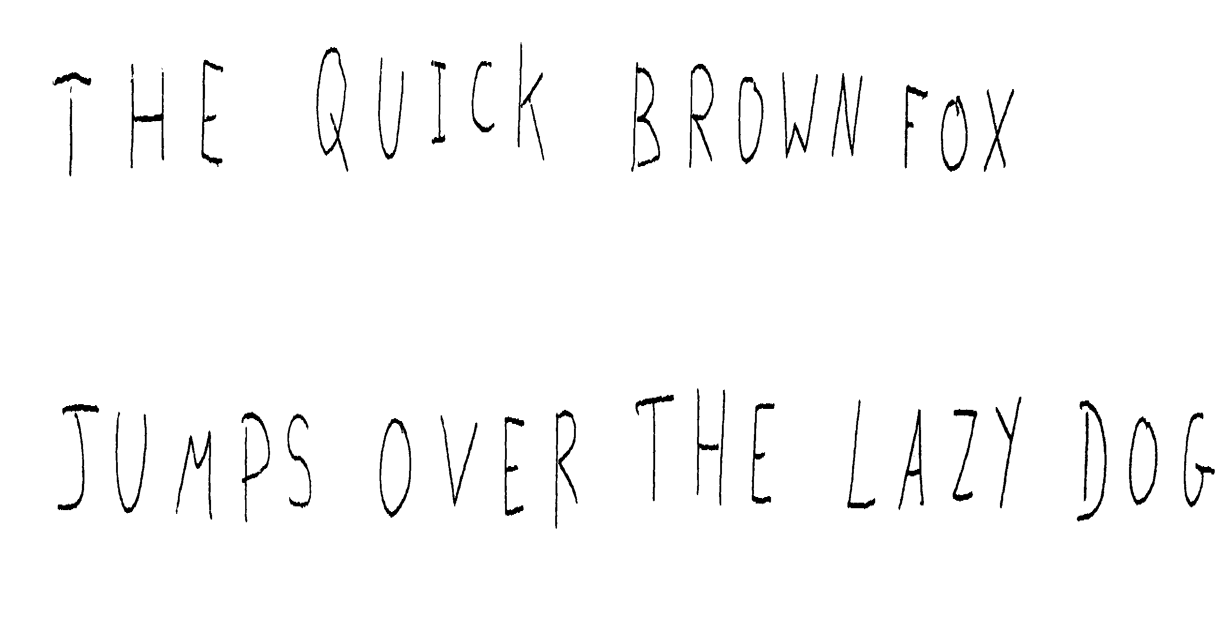
\includegraphics[width=.45\textwidth]{theBrownFox.png}
				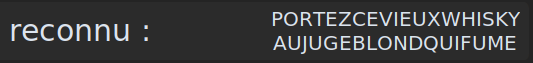
\includegraphics[width=.45\textwidth]{portezCeWhiskyLabel.png}
				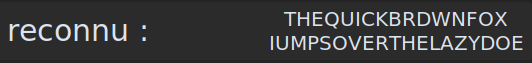
\includegraphics[width=.45\textwidth]{theBrownFoxLabel.png}
				\caption{ Pangrammes français et anglais}
			\end{center}
			\newline
			\newline
			\paragraph{} En pratique toutes les lettres sont bien reconnues. En revanche, des caractères mal écrits ou une image issue d'une binarisation médiocre rendent difficile la reconnaissance par YOLO.
			
			% \begin{figure}[H]
			% 	\centering
			% 	\includegraphics[width=0.6\textwidth]{bienMalEcrit.png}
			% 	\label{fig:bienMalEcrit}
			% \end{figure}

			\begin{center}
				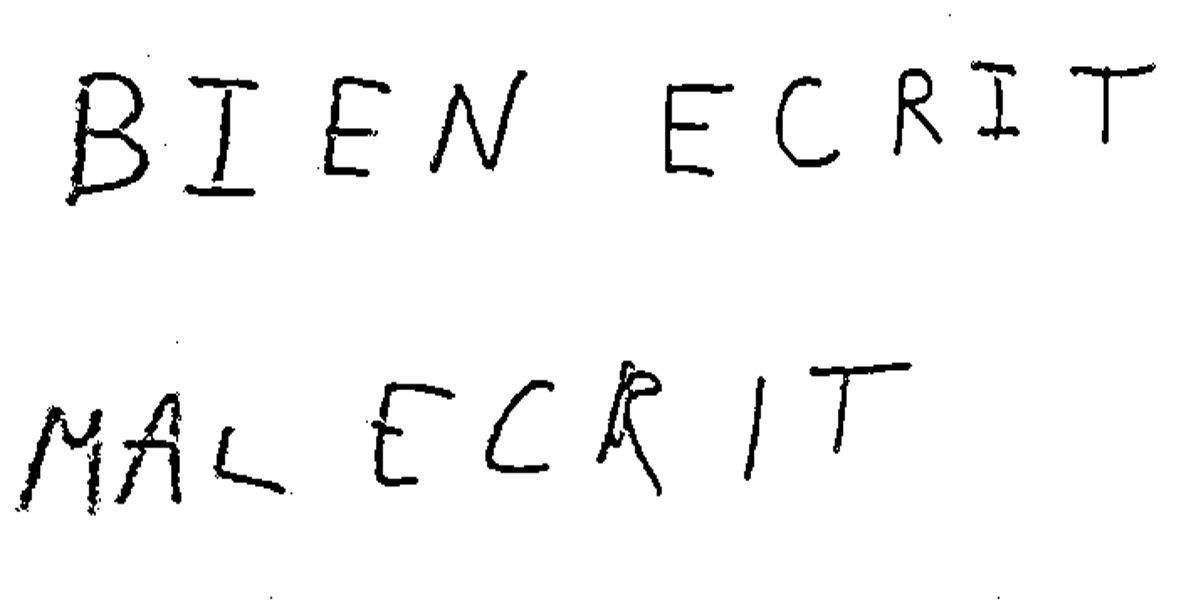
\includegraphics[width=.4\textwidth]{bienEcritMalEcrit.png}
				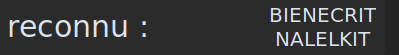
\includegraphics[width=.4\textwidth]{bienEcritMalEcritLabel.png}
			\end{center}


			\paragraph{} Grâce aux bonnes performances de YOLO, la reconnaissance d'un caractère est de l'ordre de la milliseconde. La reconnaissance se fait donc instantanément.

			\begin{figure}[h]
				\centering
				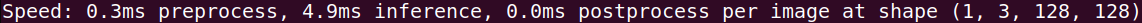
\includegraphics[width=0.95\textwidth]{speedYOLO.png}
				\caption{}
				\label{fig:speedYOLO}
			\end{figure}

	\section{Gestion du Projet}
		\paragraph{} Pendant ce projet, nous avons due communiquer et collaborer ensembles afin d'atteindre not but commun. Voici les outils que nous avons utilisé.
		\paragraph{} Premierement, pour communiquer nous avons utiliser l'application Discord. Sur lequel nous avons un groupe où nous nous envoyons des messages, des images et des fichiers.
		\paragraph{} Ensuite, pour le partage et le versioning, nous utilisons git et Github
		Laurent : filtrage, segmentation
		Romain : IHM, YOLO
		Tony : rapport
	\addcontentsline{toc}{section}{Bilan et Conclusions}%insert dans le toc
	\section*{Bilan et Conclusions}%sans numéro et pas dans le toc
		\paragraph{}
			tests
		\paragraph{}
			Cependant, certains points laissent à désirer dans notre projet. Malheureusement, une contribution de l'utilisateur est nécessaire. Pour une bonne reconnaissance des caractères, l'utilisateur doit rogner l'image. Il serait plus pratique que le \emph{rognagne soit fait automatiquement}. 
		\paragraph{}
			Ensuite, au niveau de la \emph{segmentation}, notre algorithme n'est pas capable de séparer des lettre cursives et ignore totalement les espaces.
		\paragraph{}
			Et enfin, dans le futur, le but sera que \emph{YOLO} reconnaisse aussi l'alphabet minuscule mais aussi l'alphabet français (avec les accents).
%		meilleur segmentation : segmentation des lettres cursives, reconnaissance des espaces
%		modifier les hyper paramètres de yolo
%		YOLO : lettres minuscule, avec accents
	\newpage
	\section*{Bibliographie}
		% \bibliographystyle{plain} % We choose the "plain" reference style
		% \bibliography{refs} % Entries are in the refs.bib file
	\newpage
	\section*{Annexes}
		\begin{figure}[H]
			\caption{Histogramme de projection vertical}
			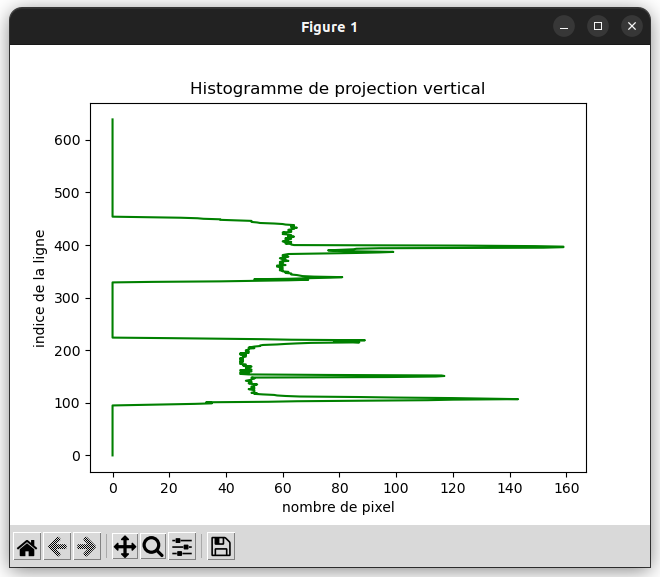
\includegraphics[width=.7\textwidth]{histoY.png}
			\centering
			\label{fig:histoY}
		\end{figure}
		\begin{figure}[H]
			\caption{Histogramme de projection horizontal}
			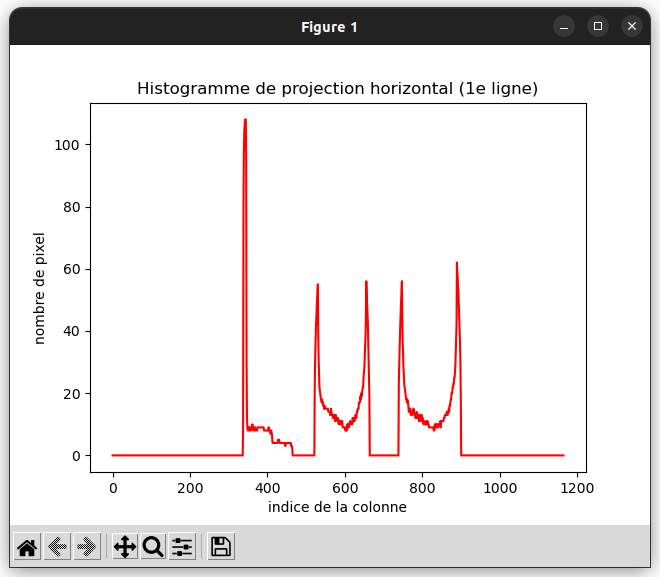
\includegraphics[width=0.7\textwidth]{histoX1.png}
			\centering
			\label{fig:histoX1}
		\end{figure}
		\begin{figure}[H]
			\caption{Histogramme de projection horizontal}
			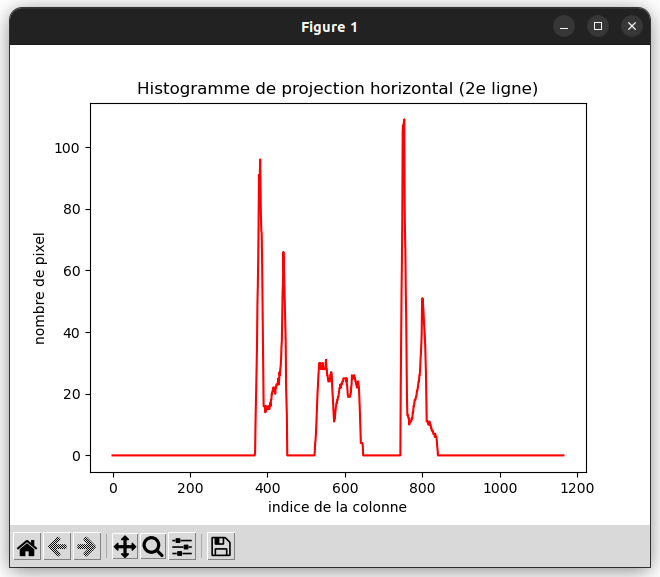
\includegraphics[width=.7\textwidth]{histoX2.png}
			\centering
			\label{fig:histoX2}
		\end{figure}
\end{document}